% This is a template designed by Maarten J. Waterloo for BSc and MSc
% students at the Faculty of Earth and Life Sciences, Vrije Universiteit
% Amsterdam, adapted to the University of Freiburg by Carsten F. Dormann. 

\documentclass[12pt,twoside,a4paper,final]{report}
% We define a two-side report on A-4 paper in final quality using a
% point size of 11 for the text. Other possibilities are {book},
% {article}, etc.

% A % sign indicates that text is commented out and will not appear in
% the document. Use \% if you want to indicate a % symbol in the text,
% thus 10\% will become 10%...

% We need to include some packages for layout and style. We do this
% below using the \usepackage command. A short explanation for each
% package is included.



\usepackage{amsmath}   % If you are going beyond the most basic level
                       % of displayed equations, you will benefit from
                       % using the amsmath package that plugs into
                       % LaTeX. This package has lots of useful
                       % features for multi-line equations, compound
                       % symbols, even commutative diagrams! Allows
                       % use \text in equations	

\usepackage{booktabs}  % booktabs is to enable the easy production of
                       % tables such as should appear in published
                       % scientific books and journals. What
                       % distinguishes these from plain LaTeX tables
                       % is the default use of additional space above
                       % and below rules, and rules of
                       % varying`thickness'.

\usepackage[top=3cm, bottom=3cm, outer=2.5cm, inner=3.5cm]{geometry}  
					   % formating the page margins

\usepackage{graphicx}  % The graphicx package implements LaTeX
                       % support for including graphics files,
                       % rotating parts of a page, and scaling parts
                       % of a page. The package depends on having a
                       % DVI driver that can produce these effects.
                       
\usepackage[hidelinks]{hyperref} %This package will make links in PDF
                       % documents to your figures, references, etc.
                       % hidelinks removes the boxes around the hyperreferenced items
                       
\usepackage[utf8]{inputenc} % Hard to explain: Define here the text encoding 
					   % used by your computer; on Linux typically utf8, on 
					   % windows ansinew and on mac often latin1;
					   % ideally, the whole world would use utf8
					   % important for öüäß (Umlaute)

\usepackage{palatino} % Use a nice serif font! Alternatives:
					   % times, palatino, ... 
					   
\usepackage{makeidx} % use this package to make an index
                       % of keywords, you have to follow this by the
                       % \makeindex command 
\makeindex             % Create the index file    
    
\usepackage[style=authoryear,backend=biber, maxbibnames=9,maxcitenames=1, uniquelist=false]{biblatex}

\addbibresource{reference.bib}

%\usepackage{natbib}    % Provides a style with author-year and
                       % numbered references, as well as much detailed
                       % of support for other bibliography
                       % use. Provides versions of the standard BibTeX
                       % styles that are compatible with natbib,
                       % plainnat, unsrtnat,
                       % abbrnat. The bibliography styles produced by
                       % custom-bib are designed from the start to be
                       % compatible with natbib.
                       
\usepackage{rotating}  % The rotating package implements three
                       % environments within which in-line figures,
                       % tables, and captions can be rotated by an
                       % arbitrary number of degrees. Two additional
                       % environments allow rotation of floating
                       % objects, which are typeset alone on separate
                       % pages.

\usepackage{wrapfig}   % allows text to flow around a figure               










\usepackage{tabularx}
% package for tables

% to isert R code
\usepackage{listings}
\usepackage[usenames,dvipsnames]{color}    

\lstset{ 
  language=R,                     % the language of the code
  basicstyle=\small\ttfamily, % the size of the fonts that are used for the code
  numbers=none,                   % where to put the line-numbers
  numberstyle=\tiny\color{black},  % the style that is used for the line-numbers
  stepnumber=1,                   % the step between two line-numbers. If it is 1, each line
                                  % will be numbered
  numbersep=8pt,                  % how far the line-numbers are from the code
  backgroundcolor=\color{white},  % choose the background color. You must add \usepackage{color}
  showspaces=false,               % show spaces adding particular underscores
  showstringspaces=false,         % underline spaces within strings
  showtabs=false,                 % show tabs within strings adding particular underscores
  frame=none,                   % adds a frame around the code
  rulecolor=\color{black},        % if not set, the frame-color may be changed on line-breaks within not-black text (e.g. commens (green here))
  tabsize=2,                      % sets default tabsize to 2 spaces
  captionpos=b,                   % sets the caption-position to bottom
  breaklines=true,                % sets automatic line breaking
  breakatwhitespace=false,        % sets if automatic breaks should only happen at whitespace
  keywordstyle=\color{RoyalBlue},      % keyword style
  commentstyle=\color{YellowGreen},   % comment style
  stringstyle=\color{ForestGreen}      % string literal style
}






% The \raggedbottom declaration makes all pages the height of the text
% on that page. No extra vertical space is added.
\raggedbottom

%----------------------------------------------------------------------------
% Allow more floating material on text pages:
\renewcommand\floatpagefraction{.9}%
\renewcommand\topfraction{.9}%
\renewcommand\bottomfraction{.9}%
\renewcommand\textfraction{.1}%
\setcounter{bottomnumber}{4}%
\setcounter{topnumber}{4}%
\setcounter{totalnumber}{4}%


%----------------------------------------------------------------------------
				% here the content starts !		
%----------------------------------------------------------------------------
% Define title and authors
\def\maintitle{The earthEngineGrabR - An R package to simplify the acquisition of remote sensing data}
%\def\subtitle{Subtitle...}
\def\authors{Janusch Jehle}
\def\supervisor{Supervisor: Carsten Dormann, Prof. Dr., Department of Biometry and Environmental System Analysis}
\def\cosupervisor{Co-supervisor: Dr.-Ing. Holger Weinacker, Department of Remote Sensing and Landscape Information Systems}
\def\year{Freiburg, May 2018}
\def\course{Master thesis  (Student ID 2920545) \\submitted to \\the Faculty of Environment \& Natural Resources \\ at the Albert-Ludwigs-University Freiburg}

% Start the document
\begin{document}

% Make some shortcuts for writing units and chemical species
% You can add your own here...
\newcommand{\mgl}{mg l$^{-1}$}
\newcommand{\mmoll}{mmol l$^{-1}$}
\newcommand{\meql}{meq l$^{-1}$}
\newcommand{\muscm}{$\mu$S cm$^{-1}$}
\newcommand{\water}{H$_2$O}
\newcommand{\kion}{K$^+$}
\newcommand{\naion}{Na$^+$}
\newcommand{\caion}{Ca$^{2+}$}
\newcommand{\mgion}{Mg$^{2+}$}
\newcommand{\clion}{Cl$^-$}
\newcommand{\nitrate}{NO$_3^-$}
\newcommand{\nitrite}{NO$_2^-$}
\newcommand{\nhion}{NH$_4^+$}
\newcommand{\hcoion}{HCO$_3^-$}
\newcommand{\hardness}{Ca$^{2+}$ + Mg$^{2+}$}


% Pagestyle of numbering, options are plain (Just a plain page number), empty (empty heads and feet - no page numbers), 
% headings	(puts running headings on each page), and myheadings (You specify what is to go in the heading with the 
% \markboth or the \markright commands.
% No numbering on title page, so we use empty here...
\pagestyle{empty}

%-- french title page (r) ------------------------------------------------
% Include the university-logo at the bottom of the page
\begin{figure}[h]
  \begin{center}
    \vspace{-2cm}
    
\includegraphics[width=4cm]{images/ufcd-logo-e1-a4-color} %ALU_longlogo}
  \end{center}
\end{figure}

\begin{center}
  {\huge\bfseries\maintitle\par}
  \vskip 2em%
%  {\Large\bfseries\subtitle\par}
%  \vskip 2em%
  {\Large\authors\par}
   \vskip 2cm%
  {\course\par}
  \vskip 1em%
   \begin{figure}[h]
     \begin{center}
       
\includegraphics[width=10cm]{images/logo_ee_croped.png}
    \end{center}
  \end{figure}
 % \vskip 2em%
\end{center}
  {\supervisor \\  \cosupervisor \\
  \flushright \year \par} 

\newpage
% If you have a photo on the titlepage, you can add a short
% explanataion here 
\begin{figure}[h]
	\begin{center}
		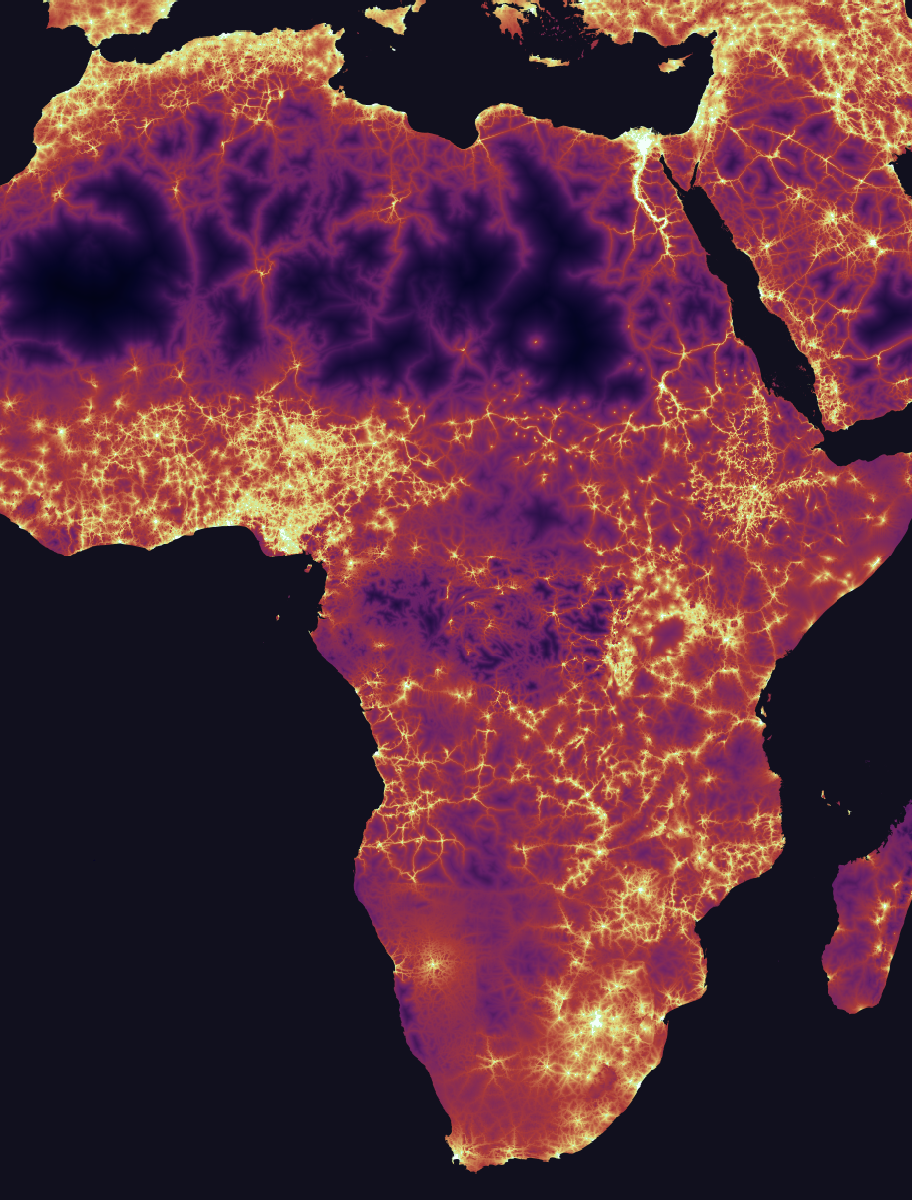
\includegraphics[width=16cm]{images/artWork_croped_2.png} %ALU_longlogo}
	\end{center}
\end{figure}
\newpage

% Page numbering, options are arabic (Arabic numerals), roman	(Lowercase Roman), Roman (Uppercase Roman)
% alph (lowercase letters) and Alph (Uppercase letters)
\pagenumbering{Roman}
\pagestyle{plain}

% Include table of contents
\tableofcontents

% Remove the % in front of the command below to include a list of tables:
%\listoftables

% Remove the % in front of the command below to include a list of figures:
%\listoffigures

\newpage
% Use arabic numbering throughout the text
\pagenumbering{arabic}

% Include an abstract of your report
\abstract{


With the decision of National Aeronautics and Space Administration (NASA), United States Geological Survey (USGS) and National Oceanic and Atmospheric Administration (NOAA), as well as European Space Agency (ESA) to provide open access to their satellite data, petabyte-scale archives of remote sensing data are now freely available.
The increasing availability, as well as the wide range of the spatial-, temporal-  and radiometric-resolution, have made remote sensing data, the best source of data for large-scale applications and studies in environmental system modelling.
Still, acquiring and preparing remote sensing data for large-scale applications is challenging and requires expertise in Geographic Information System (GIS) and access to high-performance computing resources.
Google Earth Engine is a cloud-based platform that strongly simplifies the access to high-performance computing resources while offering a multi-petabyte data catalogue of analysis-ready geospatial datasets.
By using the Earth Engine (EE) the acquisition and preprocessing of large-scale remote sensing data can strongly be simplified.

However, the EE API is accessed by a client library, whose application requires additional effort to learn. Furthermore, the client library is currently only available in JavaScript and Python. Therefore, scientists using the programming language R cannot apply the client library.

In the present work, a simplified access to capabilities of the EE for the R programming environment is presented.
The thesis aims to develop an R package - earthEngineGrabR - that simplifies the acquisition of remote sensing data by building an interface of R and EE. The interface enables to use EE as a backend-service to retrieve selected data products for a given region and time of interest in an analysis-ready format. Any acquiring and processing of the remote sensing data is entirely outsourced to EE and only the derived data products, are exported and imported into R. In a number of use cases, the earthEngineGrabR showed great potential to simplify and extend the users possibility to acquire remote sensing data for their research question. Compared to the standard approach of downloading and preprocessing the data on a local system, the earthEngineGrabR provided significant savings of time and resources while enabling the fast acquisition of processing intensive data products.


 


} 

\section{Introduction}


To model environmental systems, data about the system  and resources to process this data to derive insight, is needed. Remote sensing data, such as satellite imagery and derived data products, such as land cover, vegetation indices, elevation models, or precipitation, are integral parts of environmental system models. 
The value of remotely-sensed data as a source of input data for environmental process modeling has been increasing in the past years (\cite{melesse2007remote}). The increasing availability of remotely-sensed data from different sensors with a wide range of spatial-, temporal- and radiometric-resolution has made remote sensing data, the best source of data for large-scale applications for a wide range of study fields like urban studies (\cite{wu2000global}), hydrological modeling (\cite{bogh2004incorporating}), watershed mapping (\cite{melesse2003spatially}), energy and water flux estimation (\cite{melesse2005estimation}), fractional vegetation cover (\cite{carlson2000impact}) and drought predictions (\cite{rhee2010monitoring}).

Through contributions of several earth observation missions, the stock of freely available remote sensing data, as well as its temporal- and spatial-resolution, is continuously growing (\cite{melesse2007remote}).
However, acquiring and preparing remotely-sensed data for the use as input for an environmental system model is still related to significant expenditures of time, expertise, work and processing resources. The reason for the necessary spending is strongly related to how remotely-sensed data is acquired, stored, managed and provided.

Most geospatial environmental data is derived from satellite imagery. This primary satellite imagery is retrieved from sensors of various earth observation satellite missions that, again, are part of mainly two earth observation programmes. The most extensive programme with regards to its duration and the number of satellites is the Earth Observing System (EOS). The EOS is a cooperation of National Aeronautics and Space Administration (NASA) including various Government Agencies such as the National Oceanic and Atmospheric Administration (NOAA) and the United States Geological Survey (USGS). The second observation programm is the recent Copernicus Programm of the European Commission in partnership with the European Space Agency (ESA; \cite{salomonson2002overview}). A representative satellite mission of the EOS is the Terra satellite that carries multiple sensors and among others produces the popular imagery products: Advanced Spaceborne Thermal Emission and Reflection Radiometer (ASTER) and Moderate-resolution Imaging Spectroradiometer (MODIS). The most well-known satellite missions are probably the Landsat satellites. The Copernicus Programm at the moment has two active missions: Sentinel 1 and Sentinel 2 (\cite{butler2014earth}).
From this primary satellite imagery, a multitude of secondary geospatial environmental data like Digital Elevation Models (DEMs), land cover, atmosphere, weather, climate simulations or even socio-economic variables are derived. Examples are the National Land Cover Database (NLCD) of the USGS, the NASS Cropland Data Layers of the National Agricultural Statistics Service (USDA) but also the WorldPop project population data produced by a collaboration between researchers at different Universities worldwide (\cite{homer2007completion},\cite{johnson20102009},\cite{tatem2017worldpop}). 
As a consequence of the decision of multiple U.S agencies including NASA, USGS and NOAA, as well as ESA to provide open access to their imagery data, petabyte-scale archives of geospatial data are now freely available (\cite{gorelick2017google}).

Usually, the databases are accessible through an online search and order tool like the NASA Earth Observation, the USGS Earth Explorer or the Copernicus Open Access Hub. These tools allow searching for scenes of a remote sensing data product according to different metadata properties like acquisition time, name or spatial-coverage and order or download the selected scenes subsequently. 
Scenes are near-square images covering an area that varies in size depending on the remote sensing data. For Landsat images, the coverage is about 170 to 185 km per scene. Because these online search and order tools do not provide any processing resource, it is not possible to aggregate or subdivide the scenes to a specific extent.

\begin{center}
	\begin{figure}[h]
		\begin{center}
			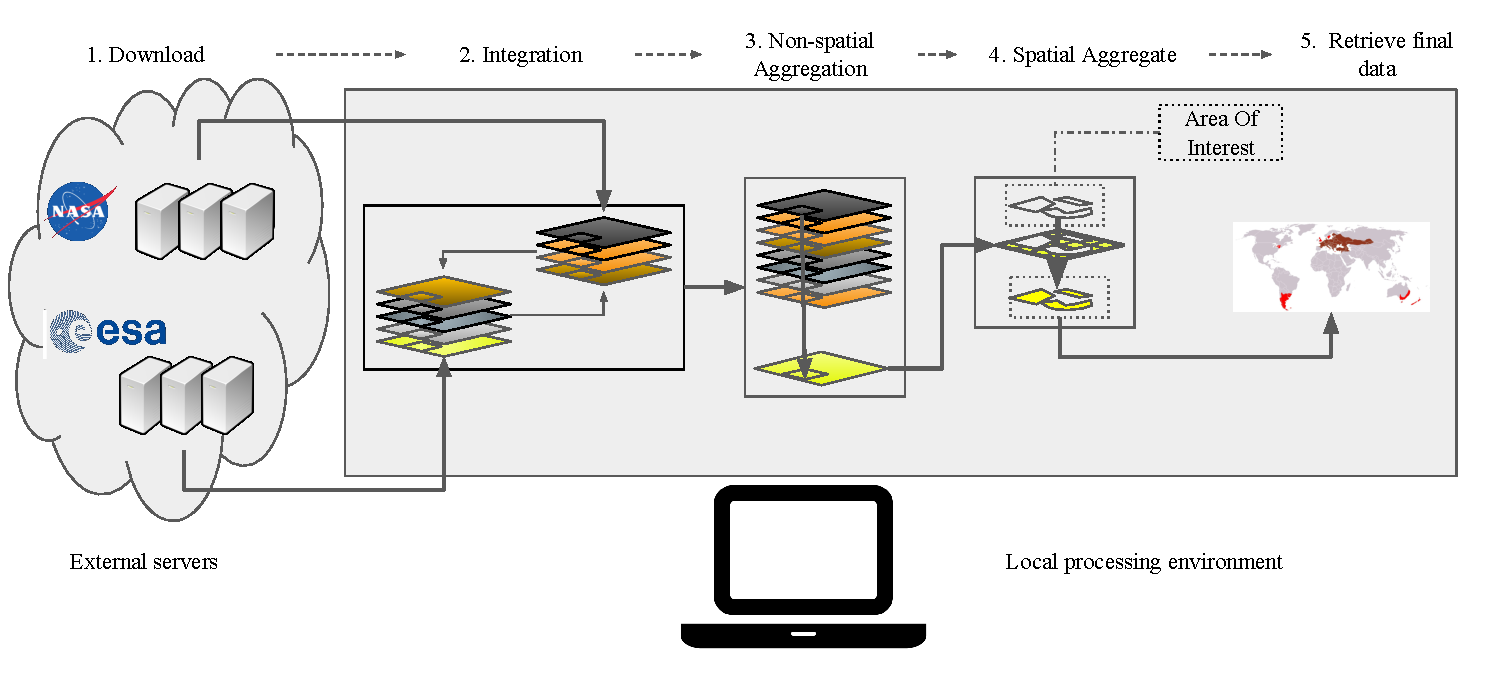
\includegraphics[width=15cm]{images/traditional_acquisition-cropped.pdf}
			\caption{Schematic approach to acquire and prepare remote sensing data for environmental system modeling}
			\label{traditionl_approach}
		\end{center}
	\end{figure}
	% \vskip 2em%
\end{center}


A standard procedure of acquiring and preparing remote sensing data comprises several steps. First, the remote sensing data must be downloaded via one of the search and order tools. If the downloaded data is acquired from multiple sensors or different sources, the different coordinate reference systems and projections need to be integrated and harmonised. Third, in case of multiple scenes of the same locations, for instance, multiple satellite images of the same location acquired at different times, the data has to be aggregated temporally. For example to calculate the yearly sum of precipitation from daily chirps satellite imagery, or to calculate the Normalised Diference Vegetation Index (NDVI) from multiple bands of Landsat imagery.
Forth, the data is spatially aggregated according to a given target. The target represents the shape of the area of interest (AOI). The AOI could be a world-wide grid of 1$^\circ$ x 1$^\circ$ cells, the resolution of a raster, a set of points representing the locations of experiments, or the sample area. Finally, in the last step, the data is retrieved as tabular data with a geographic reference (see Figure \ref{traditionl_approach}). The entire processing of the remote sensing data was performed on the local system.

The standard procedure to acquire remote sensing data is usually time consuming and cumbersome due to the interoperability and size of remote sensing data (\cite{iosifescu2011geovite}).

Because varies governments and agencies collect remote sensing data, most data are distributed and stored in different locations, in a variety of file formats, projections and resolutions. To integrate data from such diverse sources requires a manual and thus time-consuming pre-processing of the data even when processing only a few satellite images (\cite{schell2000geodata}). To perform the required integration and harmonisation of different remote sensing data sets expertise in a Geographic Information System (GIS) is prerequisite.

Furthermore, due to the limited possibility of the search and order tools to control the request to the servers, the data throughput is unnecessary high. Even though only a fraction of a scene is needed, the complete scene needs to be downloaded. Furthermore, the processing resources are not where they are needed. It is required to download the entire row data to a local system to perform the tasks necessary to prepare the data for environmental modeling. The limited control over the requested data results in many unnecessary inter-products and again raises the data throughput. While processing small geospatial data sets, this may be of no importance, but for the processing of large-scale data sets, this quickly leads to challenges in dealing with memory limitation and the necessity for big data solutions such as computer clusters or cloud computing resources.
Managing such application leads to associated challenges such as storage, management of databases and servers and managing clusters efficiently (\cite{gorelick2017google}). 

For instance, the processing of a moderately sized remote sensing imagery stack with 50 landsat satellite images (1.6 GB per image) would most likely lead to a memory limitation problems.

Hence, although petabyte-scale archives of geospatial data are freely available, the access and utilisation of these datasets for environmental system modelling are restricted due to the given difficulties. 
These obstacles hinder most researchers to make use of this massive stack of remote sensing imagery, restricting access to the information that can be derived from large remote sensing datasets, to remote-sensing experts with exclusive access to high-performance computing resources.



\subsection{}


The Google Earth Engine is a cloud-based platform that strongly simplifies the access to high-performance computing resources to process extensive remote sensing datasets, without the information technology (IT) management obstacles like, data acquisition and storage, combine different file formats, managing databases, machine allocations, CPUs, GPUs. 
Earth Engine (EE) consists of a multi-petabyte data catalogue, a high performance, parallel and therefore scaleable, computation service and is accessed and controlled through an Internet-accessible application programming interface (API). Queries are constructed by using operations drawn from the EE client library consisting of more than 800 functions ranging from simple mathematical operations to powerful geostatistical, machine learning and image processing operations (\cite{gorelick2017google}).

By using the EE the acquisition and preprocessing of large-scale remote sensing data can strongly be simplified.

EE offers an elegant solution for working with large remote sensing data and the related problems of the interoperability of the data due to distributed sources and the big data problems caused by the size of the data and required processing resources. 
Processing resources and data are connected, and there are no unnecessary inter-products or downloads. 
The data does not have to be download and preprocessed separately. Instead, the data is already stored in one managed database, pre-processed and in access and analysis-ready format. 
The computational power required to process the data is automatically scaled, which makes computations of an entirely new magnitude possible without bothering with any IT management obstacles.
With EE, it is possible to request and generate precisely the data needed for analysis, while any acquisition, integration, preprocessing and aggregation is outsourced to the EE servers. 

However, the EE API is controlled by a client library, currently only available in JavaScript and Python. To use the EE additional effort to learn and apply the client libraries is necessary, furthermore, scientists using a different programming language like R cannot access the EE API directly from within R.
There is currently no R or Python package that is using EE capabilities to simplify the acquisition and preprocessing of remotely sensed data. Actually, there is not a single R or Python package using any of EE capabilities directly. The few existing ones are written in Python and only facilitate the use of the EE API by providing a pipeline to other API's like the Planet-GEE-Pipeline-GUI or provide an automated upload feature of assets via the Google Cloud Environment like the geeadd tool (\cite{roy2017google}).

Although the Earth Engine solves many of the challenges in retrieving data from large remote sensing datasets for environmental system modeling, it is still exclusive for experienced users of the EE client library available only in JavaScript and Python.


In the following the problem statement that motivates this thesis is summaries:

\begin{itemize}
	
	\item The stack and resolution of freely available remote sensing data, as the potential as input for environmental system model, is continuously increasing.
	\item With the traditional methods discussed, the process of acquiring remote sensing data for analysis is costly and inefficient and requires high-performance computing resources.
	\item This restricting access to the information that can be derived from large remote sensing datasets, to remote-sensing experts and deviates resources from the scientific work.
	\item The EE provides a performant and flexible solution to the problems related to large remote sensing datasets and is superior to the acquisition with a search and order tool.
	\item However, the use of the EE is exclusive for experienced users of the EE client library only available for Python.
	\item Hence, to use the potential of the EE for the acquisition of remote sensing data, the access to the EE needs to be simplified.
	
\end{itemize}

The simplified access to the capabilities of EE would enable scientists to utilise the massive stack of freely available remote sensing data for their research projects without additional costs.

This work is inspired by the attempt to develop such simplified access to capabilities of the EE for the R programming environment.

The master's thesis aims is to develop an R package - the earthEngineGrabR, which simplifies the acquisition of remote sensing data for the analysis in R. This should be accomplished by building an interface between R and EE.
The interface should enable to use EE as a backend-service to retrieve selected data sets for a given region and time of interest in an analysis-ready format. The interface is supposed to extract data from the EE data catalogue while providing extensive control over temporal and spatial resolution. 
Any processing of the remote sensing data shall entirely be outsourced to the EE and only the derived data products, are exported from EE and imported in R. 

This way, the developed interface exploits two of EE's significant advantages. One is the public data catalogue of over 11 petabytes of remote sensing data in an analysis-ready format, and the other is its high-performance, intrinsically parallel computation service to process such massive data.





\section{Introduction to Google Earth Engine}

EE is a cloud-based platform that strongly simplifies the access to high-performance computing resources to process extensive remote sensing datasets, without the information technology (IT) management obstacles like, data acquisition and storage, combine different file formats, managing databases, machine allocations, CPUs, GPUs. 
EE consists of a multi-petabyte data catalogue, a high performance, parallel and therefore scaleable, computation service and is accessed and controlled through an Internet-accessible application programming interface (API). Queries are constructed by using operations drawn from the Earth Engine client library consisting of more than 800 functions ranging from simple mathematical operations to powerful geostatistical, machine learning and image processing operations (\cite{gorelick2017google}).

\subsubsection{The public data catalogue}

The majority of the EE public data catalogue consists of remote sensing imagery collected by earth-observing satellites missions from government agencies like NASA, USGS, NOAA and ESA. It contains the entire archives of Landsat, Sentinel 1-2 and Modis, but also several other environmental, geophysical and social-economic datasets. This catalogue is continuously extended and updated from current missions, and this way holds up to date satellite imagery with a latency of about one day.
In EE, imagery data or raster is stored in a 2D gridded raster container referred to as an image. One image can have any number of bands, and while each band need to be homogeneous in data type, resolution and projection, bands in an image can vary in data type, resolution and projection. Each image can have associated metadata stored as key-value pairs to provide additional information like acquisition time, location or any metadata provided.
Multiple images that are related, such as images from the same source or sensor are combined in collections. These Collections provide fast spatial and temporal filtering and sorting capabilities using metadata associated to every single image in the collection. The metadata enables users to search through millions of images to select data that meet specific criteria. For example, users can quickly filter the entire Landsat 7 archive for images within Germany, collected on day-of-year 40 - 80, from the year 1990 - 2000 with cloud cover less 50\%. While this also would be possible in one of the search and order tools, EE additionally provides extensive GIS capabilities and processing resources to further manipulate the data.
For instance, the filtered Landsat scenes could be aggregated to a median composite. The bands in the median composite could be used to calculate the Normalized Difference Vegetation Index (NDVI). The NDVI image could be spatially aggregated over multiple regions defined by the feature of a shapefile representing the states of Germany. While this process is a matter of minutes on Earth Engine, it indeed would require extended big data solutions on a local system.

What makes EE that performant is the storage system as a tile database with built-in pyramiding architecture in combination with the system architecture and several data distribution models (\cite{gorelick2017google}).

\subsubsection{The tile architecture}

Images ingested into Earth Engine are preprocessed to provide fast and efficient access. First, images are parsed into tiles in the images original projection and resolution and stored in a tile database. Each tile has the size of 256 x 256 Pixels and refers to the practical trade-off between loading unneeded data versus the overhead of issuing additional reads. Instead of resampling all data to a fixed grid, traditional data cube systems would do, this method is information-preserving (\cite{gray1997data}). Because the data is maintained in their original projection, resolution and bit depth the data degradation that is inevitable if resampling to a fixed grid, is avoided

\subsubsection{The pyramid architecture}

Additionally, a pyramid of reduced-resolution tiles is created for each image and stored in the tile database. Each level of the pyramid is produced by downsampling the previous level by a factor of two until the entire image fits into a single tile. During downsampling, continuous valued bands by default are averaged, while discrete-valued bands are aggregated using one of min, mode, max. This way, if fractions of data from an image are requested for computation in a reduced resolution, only the relevant tiles from the most appropriate pyramid level need to be retrieved from the tile database. The tile database enables EE to provide data in a variety of resolutions without introducing significant storage overhead.

\subsubsection{The system architecture}

The processing system automatically subdivides and distributes computations to enable high-throughput analysis. In EE a collection of enabling technologies is used that is available in the Google data centre environment. The Borg Cluster Management System is used to distribute and load-balance computation over multiple workers within a cluster. The FlumeJava framework is used for parallel pipeline execution of batch computations.
Users can interact with the Earth Engine by using either an associated web-based interactive development environment (IDE), third-party Web Apps, or directly with one of the client libraries on a local system by using the EE Python or JavaScript API.
The IDE code editor and the third-party Web Apps use the client libraries to send requests to EE through a Representational State Transfer Application Programming Interface (REST API). 
The Tilestore Servers houses the public data catalogue in the described architecture. In the Asset Database, the user can ingest their data. 
The Borg Cluster Management Software manages each component of the system, and each service is load-balanced over multiple workers. Failure of any individual workers results in the caller reissuing the query.

\subsubsection{Construct earth engine programmes with the client library}

The user writes EE programmes using the client library available for Python and JavaScript.
The functions in the client library can be composed to build a description of the computation the user wants to perform. This description is sent to Earth Engine servers for evaluation. To further improve performance Earth Engine uses a lazy evaluation model that allows it to compute only the fraction of output that is necessary to fulfill the current request. It postpones computing output pixels until it knows more about the context in which they are needed (\cite{gorelick2017google}).


\subsubsection{Data distribution models}

To achieve high performance, the functions in the Earth Engine library apply several built-in parallelisation and data distribution models. Each model aims to optimise a different data access pattern.
For operations that are local, image tiling is used.
In remote sensing, especially raster manipulation many processing operations are local. That is, the computation of a Pixel depends only on input pixels within a fixed distance. Examples of per-pixel operations are band math, spectral unmixing neighbourhood or convolution operations. To process operations in parallel, the area is subdivided into tiles and computed independently. This way, to process one of those tiles most of the time only a few or one input tile is needed. Image tiling combined with pyramided inputs provides a fast computation of results at any requested scale or projection.
For operations that are inherently non-local a spatial aggregations is used.
Non-local operations such as computations of regional or global statistics, raster-to-vector conversions, or sampling an image to train a classifier, can at least partly still be executed in parallel by aggregating together many sub-results. In EE, those processes are executed as distributed processes using a scatter-gather model. First, similar to the image tiling approach, a spatial region is divided into subregions that are allocated to workers in a distributed worker pool and computed independently. These intermediate results are sent back to the master of this computation, which combines them and transform the intermediate results into the final result. For instance, to compute a mean value each worker computes sums and counts, the master collects these intermediate results and compute the final results as the total sum by the total count.





\chapter{Methods}

The eartgEngineGrabR package is supposed to provide an interface of R and the EE to acquire remote sensing data in R. The emphasis is to develop a stable framework for an interface between R and the EE. This framework should enable the user to select from some data sets, choose a temporal and spatial resolution and send a request to the EE servers to process and export the data to the user's local machine. The framework is supposed to work as a foundation that eases further extensions.

The base functionality of the framework is: 
\begin{itemize}
	\item Uploading vector data to earth engine
	\item Choose from a list of data product
	\item Provide extensive control over the aggregation corresponding to the shape, temporal- and spatial-resolution
	\item Export the data products from EE and import the data into R
	\item Manage the dependencies and authentications to the involved API's
\end{itemize}

The package consists of two functions \mbox{\texttt{ee\_grab()}} and \mbox{\texttt{ee\_grab\_init()}}. The \texttt{ee\_grab\_init()} function handles authentications and the installation of additional dependencies necessary for the earthEngineGrabR package to work. The \texttt{ee\_grab()} function controlls the acquisition of the remote sensing data from EE.

First, the data section gives an overview of the data temporarily accessible through the earthEngineGrabR. 
The next section introduces the general design and functionality that the package provides during the acquisition process. The section covers how the \texttt{ee\_grab()} function can select, filter, aggregate and retrieve the requested data, while the emphasis lies on the design workflow and arguments of the function.
The following section introduces the technical framework that enables the interface of R and the GEE, while the focus in on the technical side in \texttt{ee\_grab()} function call.
The last section covers the necessary dependencies and authentications processes handled by the \texttt{ee\_grab\_init()}.

\section{Available data products}

The emphasis of the current version of the earthEngineGraR package is to develop a stable interface of R and the GEE to retrieve data in a user-specific form. Therefore the temporally available data is still limited to a selected list of data products, that should illustrate the diversity of the EE data catalogue. In the further development of the earthEngineGrabR package, this list should be extended.

\begin{table}[h]
	\begin{tabularx}{\textwidth}{|l|l|X|X|X|}
		\hline
		\textbf{data source} & \textbf{data product} & \textbf{spatial} & \textbf{temporal} & \textbf{availability}\\
		\hline
		
		MOD44B.051 & Tree-cover  & 30 m & yearly & 2000–2015 \\
		
		& Non-tree cover  & 30 m & yearly & 2000–2015 \\
		
		& Non-vegetation  & 30 m & yearly & 2000–2015 \\
		
		JRC SW  & Distance to SW & 30 m & yearly & 1984–2015 \\
		
		CHIRPS & Precipitation & 0.05$^\circ$ & yearly & 2000–2015\\
		
		SRTM & Elevation  & 30 m & single & 2000\\
		& Slope  & 30 m & single & 2000\\
		
		Oxford MAP & Accessibility to cities  & 0.01$^\circ$ & single & 2015\\
		
		& Friction surface  & 0.01$^\circ$  & single & 2015\\
		
		\hline
	\end{tabularx}
	\caption{Data products with temporal coverage, temporal- and spatial-resolution available in the earthEngineGrabR}
	\label{data}
\end{table}

Table \ref{data} shows the data products temporally accessible through the package. In the following, it is distinguished between a data source of the remote sensing data, that represents the primary source, for example, the Modis MOD44B.051 Terra Vegetation Continous Fields (VCF) and the derived data product: percent tree cover. In the earthEngineGrabR, the user requests remote sensing data as specific data products. A data product always represents one band of the source satellite image and one environmental variable like percent tree cover, distance to surface water or slope.
The variables vary in temporal and spatial resolution dependent on the data product they are derived from. 

To access land cover, the MOD44B.051 Terra VCF product with a yearly temporal resolution and a 250 m spatial resolution is used. The data set provides a sub-pixel-level representation of surface vegetation cover, designed to continuously represent earth's terrestrial surface as a gradient of three essential surface cover components: percent tree cover, percent non-tree cover and percent bare. The data set is generated using monthly composites of Terra Modis 250 m and 500 m Land Surface Reflectance data (\cite{hansen2006vegetation}).
The Joint Research Center (JRC), Water Classification History, is a data set, produced in collaboration with the European Commission and Google. The data set provides a pixel-wise classification of surface water generated using, 3,066,102 scenes from Landsat 5, 7 and 8 acquired between 1984 and 2015. Each pixel was individually classified into water and non-water. The data comes in an original monthly temporal resolution and an aggregated yearly resolution. In the earthEngineGrabR, the aggregated yearly water classification data is used, providing a pixel-wise classification of seasonal water, permanent water and not water (\cite{pekel2016high}). To convert this information in an ecological context, the data is further processed to receive the distance to surface water (SW) product for each pixel. To compute the distance permanent and seasonal water are merged. Therefore the distance refers to permanent and seasonal water.

To provide topographic products, the Shuttle Radar Topography Mission (SRTM) of NASA acquired in 2007 with a spatial resolution of 30 m, is used. While the SRTM dataset provides elevation in meters, the slope product is additionally processed in EE (\cite{farr2007shuttle}). To account for socio-economic variables the recently published Oxford MAP datasets of Accessibility to Cities for 2015 and Global Friction Surface for 2015 both with a spatial resolution of 0.01$^\circ$, what corresponds to approximately 30 m, are used. The global Friction Surface map estimates land-based travel speed for land pixels in the year 2015, and the global Accessibility map estimates land-based travel time to the nearest densely-populated area for the year 2015. Both datasets were produced through a collaboration between the Univerity of Oxford Malaria Atlas Project (MAP), Google and the European Union JRC (\cite{weiss2018global}). To produce the maps, the first time a global-scale combination of Open Street Map data and Google roads dataset was used, extended with datasets for topographic conditions, land cover types and national borders.
For the Friction Surface map, these underlying datasets were used to calculate travel speed regarding time to cross each pixel, with the fastest travel mode intersecting the pixel being used to determine the speed to travel in that pixel. The travel speed is in minutes required to travel one meter. The Accessibility map is produced by using the Friction Surface map in combination with a least-cost-algorithm, which calculates the travel time in minutes for each pixel to the nearest city. Cities were determined by using data from the Global Human Settlement Project.  

The Climate Hazard Group InfraRed Precipitation with Station Data (CHIRPS) is a global rainfall data set with a daily temporal resolution and 0.05$^\circ$ spatial resolution (approximately 150 m) (\cite{funk2015climate}). In the earthEngineGrabR, the CHIRPS daily (version 2.0 final) is utilised, an aggregated version of the daily CHIRPS dataset, with a temporal resolution of 1 days.

For consistency, the data products that have a high spatial resolution like CHIRPS and JRC are only available between 2000 and 2015. This way, there is one corresponding period most data is available in.

\section{Design and functionality of the \\ data manipulation}

As described in the introduction, the necessary preprocessing of the remote sensing data is an integral part of the data acquisition process. In the earthEngineGrabR, the complete integration and aggregation of the data are outsourced to EE.
Instead of downloading the raw raster data the package provides control to filter and aggregate selected data products according to a given target. This processing allows retrieving the data products in a specific, user-defined format. The user specifies a data product with a corresponding time interval and a temporal reducer, a spatial reducer and a target. 

A data product in the earthEngineGrabR is specified with a earth engine data product-function. Each function specifies one particular data product with the corresponding parameters. The name of the function is \texttt{eeProduct\_ } followed by the source of the data products, underscore the name of the data product. For example: \texttt{eeProduct\_modis\_treeCover()}. The output of the function is simply an object of the class list that specifies the parameters of the requested data product. To use a function, that produces the required parameters instead of committing a list or a vector with the listed parameter, holds several advantages illustrated in the result section.

In the EE a reducer is a way to aggregate data over space and time. In the earthEngineGrabR, there are implementations for simple statistics like mean, mode, max, and min. The temporal reducer aggregates the data over time and the spatial reducer aggregates the data over a region defines by the target. 
The target is defined by vector data, where the spatial extent of the features define the region the spatial reducer is applied over.

\begin{center}
	\begin{figure}[h]
		\begin{center}
			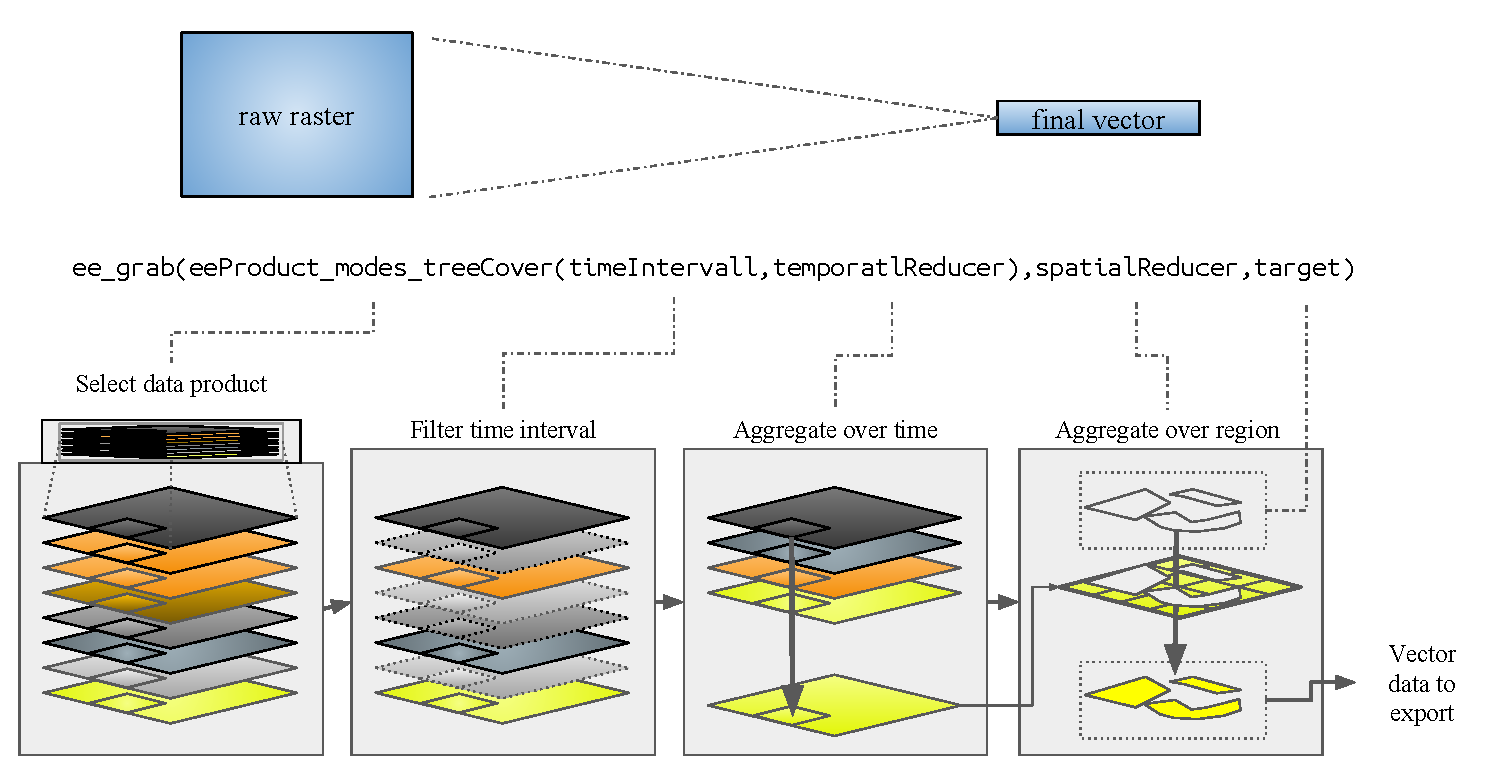
\includegraphics[width=15cm]{images/design_function-cropped.pdf}
			\caption{Function design and the data manipulation workflow of the ee\_grab function}
			\label{Workflow}
		\end{center}
	\end{figure}
	% \vskip 2em%
\end{center}

Figure \ref{Workflow} shows the basic processing flow to acquire the modis-tree-cover product for a defined time interval and a specific region. First, the data product is selected, with the corresponding data product function. If the data has a temporal resolution, the time interval as the temporal reducer is set inside the data product function. The time interval is used to filter the collection of the source data set. The images passing the filter are reduced to one image with the given temporal reducer. Next, for each region of the reduced image, which overlaps with a feature in the target vector data, a reducer is applied, and a statistic is computed. This enables the user to temporally and spatially aggregate the remote sensing data in a strongly user specific and flexible approach. The final data is returned as vector data.
The output of the \texttt{ee\_grab()} function is an object of class sf. The sf package provides a convenient approach to work with vector data in R and tries to succeed the widely used sp package in the future (\cite{sf}). An sf object is a data.frame with an additional geometry list-column, what strongly simplifies manipulating an sf object by filtering, selecting or summarising. 
During this entire processing flow, the size of the data is massively reduced, while the data is converted from a large remote sensing datasets in raster format to highly flexible and small vector data. The reasons to use vector data instead of raster data and the corresponding advantages are explained in the discussion.


\section{Technical framework}

To enable R users to request and download data from the EE, the package combines multiple tools like the programming languages R, Python, as well as multiple web services provided by Google like the Fusion Tables, Google Drive and of course the EE. While Google Drive is a general file sharing and storage service for all kinds of files, Google Fusion Table is specifically designed to manage tabular data and enables to upload, manipulate, visualise and share small amounts of data online.

Each tool performs a specific task. In R, the user specifies the requested data and initialises all further processes. In Python, the actual request is generated and send to EE. Because EE can import Fusion Tables, the Google Fusion Table is used to upload local vector data to EE. The EE performs all data processing and exports the data to Google Drive wherefrom it is downloaded and imported into R. 

\begin{center}
	
	\begin{figure}[h]
		\begin{center}
			\includegraphics[width=15cm]{images/processin_folw.pdf}
			\caption{Internal processing flow of the \texttt{ee\_grab()} function call}
			\label{processingFlow}
		\end{center}
	\end{figure}
	% \vskip 2em%
\end{center}

Figure \ref{processingFlow} describes an internal processing flow of the \texttt{ee\_grab()} function.
At the beginning of the function call, the target vector data is uploaded as Fusion Table illustrated with the dark yellow arrows with number 1. 
The group of processes with the number 2 in red, describes the integration of R and Python and the method Python code is executed from R. The processes with number 3 in yellow, represents the exchange of arguments, or,  how parameters are passed from R to Python. The orange arrows with the number 4 illustrate the structure of the Python code as executable modules. The blue processes with the number 5 show the communication of the Python client library and EE while the dark blue arrows with number 6 describe the approach to send process info from EE to R. In dark grey with number 7 the import of the Fusion Table, the computation and the export of the processed data is illustrated and finally the green processes with number 8, describes the access from R to Google Drive and the following download and import of the final data into R.
Based on the classification of the flowchart of figure \ref{processingFlow}, the following section explains all eight groups of processes in detail.

If installed, the eartEngineGrabR R library is located in a default library folder for all R libraries. In the eartEngineGrabR folder, there is R folder, containing an R script, which defines all R functions used in the package. Furthermore, there is an additional Python folder containing Python scripts divided into execution scripts and function scripts. The function script, again, defines all Python functions. The execution Script, however, is executed from R and uses these functions.

To upload the target vector data the Fusion Table driver in the Geospatial Data Abstraction (GDAL) library is used. To execute GDAL from R, R's ability to invoke function calls is applied. This method will be explained in more detail in the following section. GDAL's \texttt{ogr2ogr()}  function handles the upload process, that converts a variety of geo file formats to a Fusion Table. In Fusion Tables, geometries need to be expressed in the World Geodetic System 1984 (WGS84). Therefore the projection of the vector data uploaded as Fusion Table is converted and if necessary needs to be reprojected in EE.
The EE is accessed with the EE client library available for Python. To access the EE from R it's necessary to execute Python from R. The integration should enable to pass arguments from R to Python and execute Python code from R. Instead of using a Python wrapper for R like the rPython package, earthEngineGrabR utilizes a simple command line or terminal to execute one language from the other, illustrated by the red arrows with the number 1. The \texttt{ee\_grab()} function defined in the R script functions.R, in red, invokes a system call by utilising the command line that executes the python execution script (execution.py) and simultaneously, in yellow with the number 2, passes the parameters, to the execution scripts by using a flat file. 

\begin{center}
	\begin{figure}[h]
		\begin{center}
			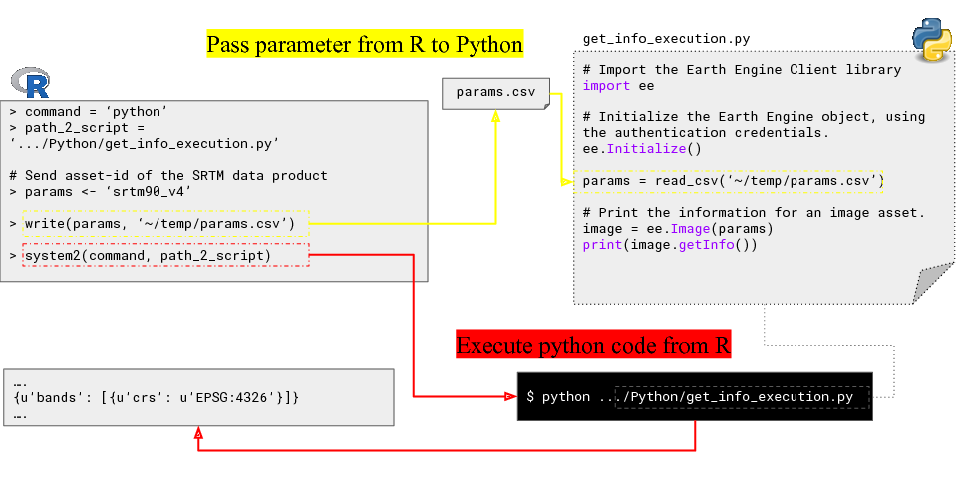
\includegraphics[width=15cm]{images/concole_connection-cropped.pdf}
			\caption{Example of utilizing the console to execute a Python script from R, that requests metadata on the SRTM data set on EE}
			\label{consoleConnection}			
		\end{center}
	\end{figure}
	% \vskip 2em%
\end{center}


To illustrate this two processes in practice, figure \ref{consoleConnection} shows a simplified code example of how to retrieve metadata of a specified data product from EE in R with the command line as the connection of R and Python. The figure presents how to execute Python code from R in red and how to pass parameters from R to Python in yellow. The left boxes illustrate the R console, the right box the Python execution script and the black box the command line.
In R the \texttt{system2()} function of the base package invoices system commands and additional arguments in all operating systems. 
To run the python script \texttt{get\_info.py}, the system call simply consists of the command \texttt{python}, to open the Python interpreter and the path to the Python script. The \texttt{system2()} function then produces the system call in the command line shown in the black box and runs the \texttt{get\_info.py} script. To pass parameters from R to Python a flat file connection is used. The Parameter is defined in R, then written to a CSV file and read again into the execution script. In this example, the parameter is the asset-id of the SRTM data set in EE. 
In the Python script \texttt{get\_info\_execution.py}, first, the EE client library is imported and initialised with the authentication credentials then the parameters are imported. To load the SRTM data product from the EE data catalogue, the asset-id is put inside an EE object (\texttt{ee.Image()}) specifying an image. To access metadata from this EE object their \texttt{getInfo()} method is called and put inside a \texttt{print()} statement. The output of this script is the output of the print statement. This output is formatted in JSON and in the default setting of the \texttt{system2()} function, the output is directly printed to the R console. Although simplified, this example shows the essential integration of R and Python and the approach to send parameters. 

\subsubsection{Sending parameters}

Although it would be possible to send parameters directly over the command line, with an increasing number of parameter, this method becomes confusing and error-prone due to text formatting differences of the command line dependent on the operating system. Therefore the package utilises a flat file connection that provides a reliable method for exchanging parameters independent from the operating system.

\subsubsection{Organize Python code os modules}

All necessary processing of the data in EE is described with the EE client library in Python. To maintain a well-arranged structure, the code is organised like a sub-package, inside the earthEngineGrabR package. There is an execution script, executed with the method described above, that calls functions defined in a Python script (functions.py). This relationship is illustrated in figure \ref{processingFlow} with the orange arrows with number 3, that appears as a circle. This Python script defines all functions necessary for the data manipulation workflow shown in figure \ref*{Workflow}. The functions are organised like independent modules, each describing one process in the processing chain shown in figure \ref*{Workflow}. There are functions for temporal filtering and reduction, spatial reduction and export. The modules take the parameters as function arguments, and this way provide the described control over the requested data.

\subsubsection{Use of the client library}

The client library consists of objects, which represent placeholders for data types stored on the EE servers, each object has corresponding methods or functions that manipulate this data type. Figure \ref{consoleConnection} showed an example of an EE object for an Image. To perform a computation in EE, the objects and corresponding methods are composed and combined to build a description of the computation the user wants to perform. 

\subsubsection{Communication of the client library and EE}

At the moment the script is executed, this description is sent to the EE servers through a REST API, in figure \ref{processingFlow} indicated as a blue arrow with the number 4. REST is a web service often used to request and modify data on a server through a Hypertext Transfer Protocol (HTTP).
In the context of the EE client library, it refers to using HTTP verbs to retrieve and modify representations of data stored on Google's servers.
In a REST system, resources are stored in a data store. A client sends a request that the server performs a particular action (such as creating, retrieving, updating, or deleting a resource), and the server performs the action and sends a response. In the case of the earthEngineGrabR package, the request is: import a specific data product, filter a time interval, aggregate over time, aggregate over regions and export the generated data to Google Drive (in figure \ref{processingFlow} as a dark grey arrow with number 6). While this is the action of the request that is performed the response of the request is to send info about the export process, in figure \ref{processingFlow} represented as a dark blue arrow with number 5. This process info includes metadata of the exported object and whether the export was successful or not. To send this info to R again a flat file connection is used, because the response is in JSON, the info is written to disk as a JSON file and afterwards imported into R. The last step in the processing chain is to access Google Drive from R and first download and next import the data into R (shown as green arrows with number 7). To access Google Drive from R, the googledrive R package is used. The googledrive package enables selection and download of specific files stored on the users Google Drive account. To identify the files to download, the metadata included in the retrieved process info is used. First, the data is downloaded in the temp folder that corresponds to the current working directory and if available on disk imported into R.

\subsubsection{Parallel processing of data products}


To process multiple data products in a \texttt{ee\_grab()} function call, each data product is processed in an individual request to the EE servers. While the upload of the target vector is performed only once, the remaining seven processes of the processing flow in figure \ref{processingFlow} are iterated for each data product. This approach allows the parallel processing of the data products. The individual requests for the data products, generated by the EE client library in Python, all end with a command to export the generated data to Google Drive (in figure \ref{processingFlow} shown as green arrows with number 7). However, the request must not wait until the data is processed and exported to Google Drive. Instead, the request ends with the response of the EE servers, whether EE started the processing. 
This allows requesting the computation of multiple data products at the same time. The exported data products are individually downloaded from Google Drive and finally joined in R.


\section{Organize dependencies and authentications}


The earthEngineGrabR package has several package dependencies in R and Python. While most R dependencies can be handled within the description file of an R package, the Python dependencies need to be manually installed with a package manager like pip. Furthermore, the package connects to several API's, which each require an individual, user-specific, authentication procedure. Therefore, a user-friendly organisation of all requirements of the earthEngineGrabR to work is particularly important. To leave the installation of dependencies and authentications to the user, would significantly hinder the use of the package and make it more cumbersome. 


To simplify the installation and authentication process, the earthEngineGrabR includes a function \texttt{ee\_grab\_init()} that installs Python dependencies and furthermore guides the user through the different authentications. Before using the earthEngineGrabR, the user has to call \texttt{ee\_grab\_init()}. 

\subsubsection{Dependencies}

Table \ref*{dependencies} lists the different dependencies for the earthEngineGrabR and how they are installed. 

\begin{table}[h]
	\begin{tabularx}{\textwidth}{|X|C|C|}
		\hline
		\textbf{library} & \textbf{dependency} & \textbf{installation}  \\
		\hline
		googledrive & R  & description file  \\
		dplyr & R  & description file  \\
		rjson & R  & description file  \\
		sf & R  & not provided  \\
		GDAL & R, Python  & not provided  \\
		google api python client & Python  & setuptools  \\
		pyCrypto & Python  & setuptools  \\
		earthengine-api & Python  & setuptools  \\        
		pandas & Python  & setuptools  \\        
		json & Python  & setuptools  \\        
		\hline
	\end{tabularx}
	\caption{Library dependencies of the earthEngineGrabR and how the installation is handled}
	\label{dependencies}
\end{table}

The dependencies handled by the description file are automatically installed during the installation of the earthEngineGrabR, while the libraries dealt with the setuptools utility are installed with \texttt{ee\_grab\_init()}. The installation of sf and GDAL is not provided and has to be manually installed by the user prior to the use of the earthEngineGrabR.

The earthEngineGrabR depends on a Python version higher 2.7 with python path set (PYTHONPATH). To ease the installation of the Python dependencies, all dependencies are combined in a new python package (GEE2R), using the setuptools package in Python. The GEE2R Python package can then be installed with the package manager pip. During this installation, all specified python dependencies are installed at once. This process is similar to the use of the description file in R packages. To call pip from R, R's described ability to invoke a system call with the \texttt{system()} or \texttt{system2()} function is used.

\subsubsection{Authentication}

In the earthEngineGrabR, three APIs are used. The EE API, the Google Drive API and the Google Fusiontable API. Each API require an authentification with a valid Google account, and concerning the Google Earth Engine API, a Google account activated for EE use. According to Google, the EE is free for research, education and nonprofit use furthermore results of the analysis performed by the user, as well as new algorithms wrote by the user remain in the property of the user alone (\cite{terms}).
To get access to EE the user has to fill out a form and wait until the request for excess is granted. If the excess is granted the user's Google account activated for excessing EE. For utilising the Google Drive API and Google Fusiontable API, only a valid Google Account is necessary. All API's use the OAuth 2.0 Protocol to manage the authentication process. To send a valid request to one of these APIs, the request needs to be authorised with a valid access token generated with the OAuth 2.0 protocol (\cite{hardt2012oauth}). To manage the OAuth 2.0 protocol and generate these tokens the earthEngineGrabR package uses different approaches depending on how each API is accessed. 

The initial call of the \texttt{ee\_grab\_init()} guides the user through the different authentications. The \texttt{ee\_grab\_init()} function only needs to be called once, and the required authentification tokens are saved and managed independently. 







\chapter{Results}

The following section is supposed to provide a scientific scenario and three corresponding sample sessions in which the earthEngineGrabR can be used to acquire remote sensing data to meet a specific question. The emphasis of this section lies on how to use the earthEngineGrabR and gives tips and tricks on how to apply the package.

\section{Szenario}

Imagine, you are a scientist involved with the MIKE Programm (Monitoring the Illegal Killing of Elephants). 


\begin{wrapfigure}{r}{0.5\textwidth}
	\begin{center}
		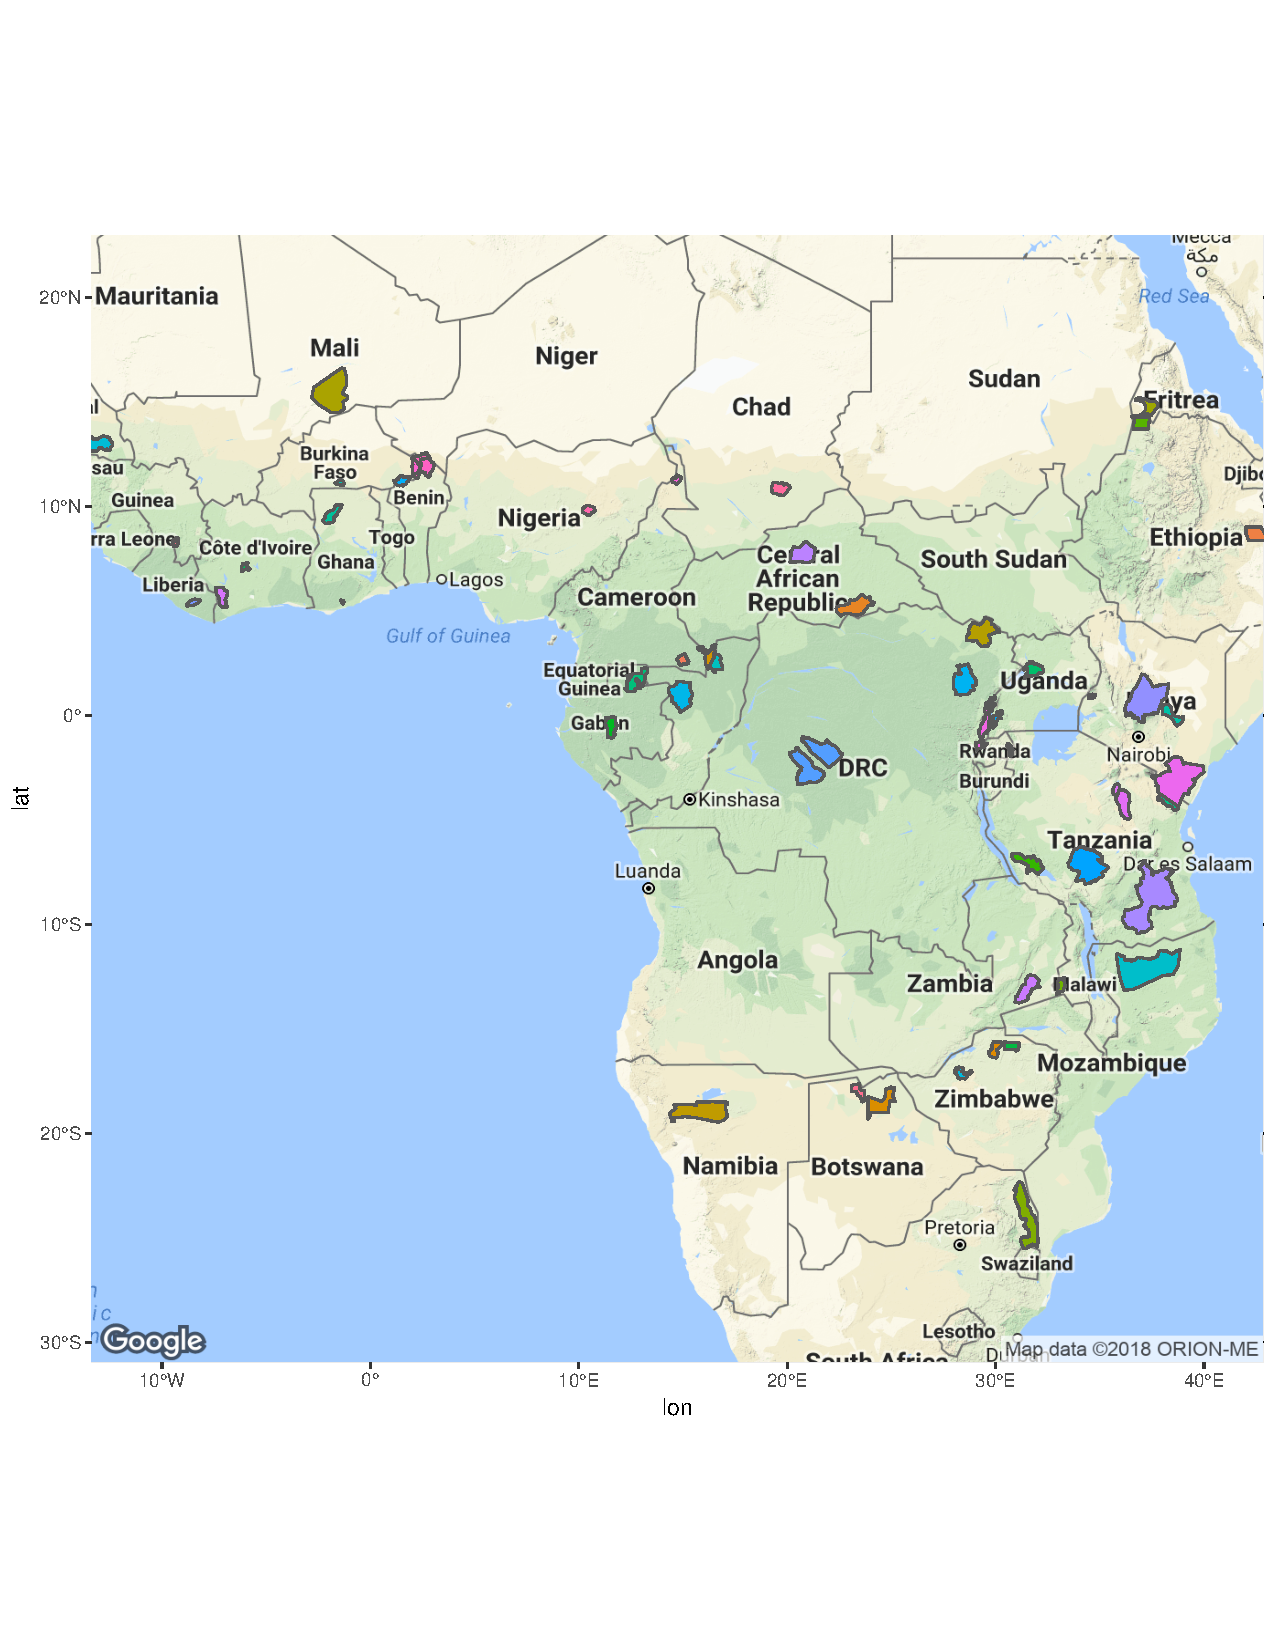
\includegraphics[width=7cm]{images/territories.pdf}
	\end{center}
	\caption{Elephant territories for the Great Elephant Census aerial survey}
	\label{territories}
\end{wrapfigure}
% \vskip 2em%

Your object of investigation is to find covariates for the intensity of illegally killed elephants in Africa. You have access to data collected within the Great Elephant Census, a continent-wide aerial survey counting the number and distribution of elephants within there territories. Figure \ref{territories} shows the study area. Each region corresponds to a territory, and for each territory, you have the aggregated number of illegally killed elephants. To run your statistical model in R and find influential covariates you need further environmental variables derived from satellite imagery like the topography, land-use, and precipitation. 


Because the study area is fragmented and of large-scale at the same time it would require significant effort to use one of the search and order tools like the Earth Explorer, to acquire and prepare the remote sensing data for your analysis. You would have to download a multitude of tiles for each of your environmental variables to cover the study area. Next, you would have to integrate, merge and aggregate all this data in an external GIS application before you start your actual analysis in R. But fortunately, you know, that one of your colleagues lately used a new R packages, some "graber" that greatly simplified his data acquisition process and you are desperate enough to give it a try. After some googling, you find the earthEngineGrabR and the corresponding Git Hup page, which describes how to apply for an EE account and how to install the required dependencies for the package. Because you have GDAL and Python already installed, you only install the sf R package and wait a few hours for the acknowledgement e-mail from Google, that you or your Google Account is now a trusted tester of the EE. Now you are ready to use the earthEngineGrabR.

\section{Large-scale analysis}

First, install the package from Git Hup with the \texttt{install\_githup()} function form the devtools package.

\begin{lstlisting}
library(devtools)
install_github("JesJehle/earthEngineGrabR")
\end{lstlisting}

After installing the package the first step is to initialize the package with \texttt{ee\_grab\_init()}. 

\begin{lstlisting}
library(earthEngineGrabR)
ee_grab_init()
\end{lstlisting}

As described in the method section the \texttt{ee\_grab\_init()} function installs all additionally required dependencies and guides the user through the authentication processes to activate the different API's. To authenticate to the API the user has to log in to his Google account and allow the API to access data on googles servers on the user's behalf. 


If the Google account is verified and the permission is granted, the user is directed to an authentification token. This token is manually copied and pasted into a running command line script, which creates persistent credentials. Later, the credentials are used to authenticate a request to the API. To simplify this procedure, the \texttt{ee\_grab\_init()} function successively opens a browser window to log into the Google account and a corresponding command line window to enter the token (see figure \ref{install}). 

This process is repeated for each API. If the function runs successfully, all needed credentials are stored for further sessions. Because some of the credentials expire after a few hours, a reauthentication is necessary. This process is handled automatically inside the \texttt{ee\_grab()} function. If a reauthentication is needed the function opens a browser window and the user is asked to log in to his Google account. The creation of credentials is automated, and there is no need to copy or paste the token manually.

\begin{center}
	\begin{figure}[h]
		\begin{center}
			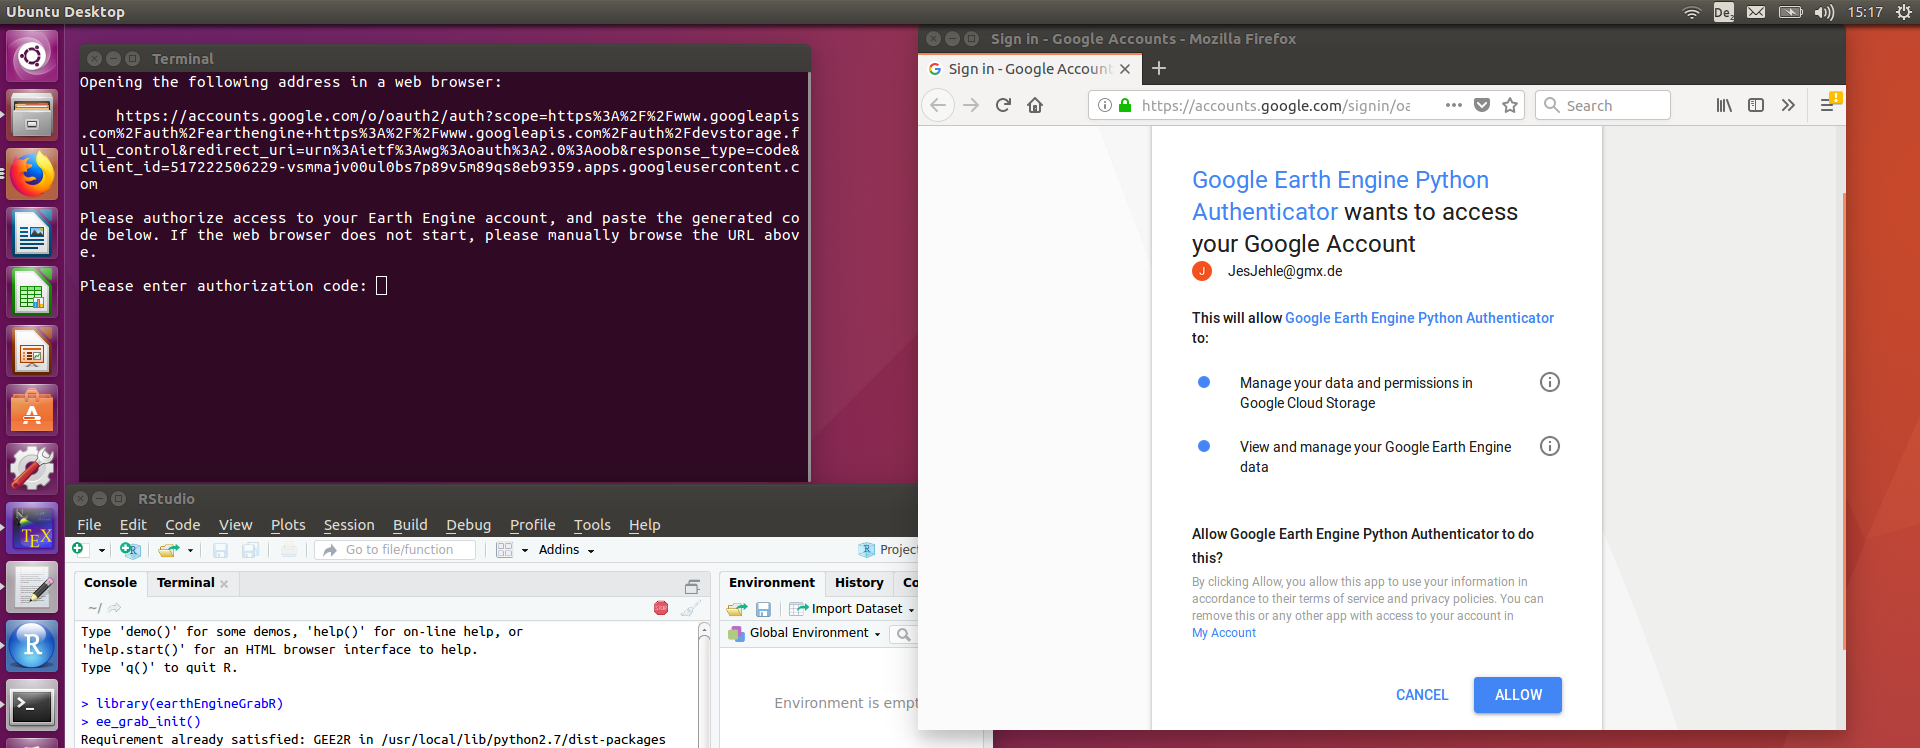
\includegraphics[width=15cm]{images/install_authentication.png}
			\caption{Example of the authentication process for the EE API}
			\label{install}
		\end{center}
	\end{figure}
	% \vskip 2em%
\end{center}



To acquire the data next the \texttt{ee\_grab()} function is used. The target is the path to the shapefile of the elephant territories shown in figure \ref{territories}. The products argument takes a list of earth engine data product-functions. Each function specifies one particular data product, and it's necessary parameter. The name of the function is \texttt{eeProduct\_ }followed by the source of the data products, underscore the name of the data product. For example: \texttt{eeProduct\_modis\_treecover()}. Because all data products start with \texttt{eeProduct\_ }, by simply typing \texttt{eeProduct\_ }, R's autocomplete function opens a drop-down menu of all available data products. Furthermore, the selection of a product in the menu displays a little description of the product and list their possible parameters. For more Information on a particular data product simply open the documentation of the function by pressing F1, or use equivalent methods. This way, it's possible to browse through the products, without any additional metadata outside of R. Additionally the functions provide default parameter values, which allow a test run without the need of specifying any parameter. While this procedure provides a user-friendly selection of available data products with their corresponding parameters, it also minimises potential typing and spelling errors.

After browsing through the data products, you choose the modis-tree-cover product for the year 2000 to 2005. You are further interested in the mean tree cover between this period and also want the mean tree cover in each of the elephant territories. Because the default value for the time reducer and the spatial reducer is mean you only need to specify the time interval parameter with a vector of the start and end-year (\texttt{timeInterval = c(2000, 2005)}). You are further interested in a potential correlation of the accessibility to populated areas and the illegally killed elephant. Therefore you additionally choose the oxford-accessibility product. The information displayed by the R's auto compete feature reveals only one possible parameter - spatialReducer - and by requesting the documentation of the function, you learn that this data product is only available for the year 2015, and therefore has no temporal resolution to aggregate. Again, you choose the mean accessibility in each territory by using the default value of the parameter and add the product function to the list. The last argument specifies the resolution in meters as edge length. 


\begin{lstlisting}

africa_elephant_data <- ee_grab(
target = system.file("data/territories.shp", package="earthEngineGrabR"),
products = list(
eeProduct_modis_treeCover(yearIntervall = c(2000, 2005)),
eeProduct_oxford_accessibility()
),
resolution = 1000
)
\end{lstlisting}


The resolution parameter sets the resolution of the processed data in EE and applies for all products. A value smaller than the native resolution of the data product results in EE resampling the data with the default nearest neighbour method, values higher result in a pixel aggregation with a default method mean. In the documentation, you learned that the native resolution of the tree cover product is 250 m while the accessibility products provide a resolution of 30 m. Because the area of the elephant territories is of large-scale (mean area of the regions is 9862 km$^2$), you choose 1000 m as the scale of your analysis. The resolution parameter actively controls the scope of computation and out of this the processing time. Therefore it's a good choice to not unnecessarily set him too low. 
Since all parameters are set, the function can be executed. 
During the processing the function prints info corresponding to the state of the upload, the processing and the download of each data product. With the verbose = FALSE, this behaviour can be avoided. 

As most processes of the function call are performed on Googles servers, the execution time depends strongly on the throughput of your analysis on the servers and only slightly on the performance of your local machine. However, because of the upload and download process during the function execution, deficient internet speed (1 Mbit/s in download and 0.1 Mbit/s in upload) can work as a bottleneck, particularly during the upload process. 
On a 64-bit ubuntu machine with 8 Gbit of RAM, 4 cores with 2.40 GHz and internet speed of 10 Mbit/s in download and 1Mbit/s in upload the \texttt{ee\_grab()} function took 55 s to execute. All further time measurements refer to this setting.
The output of the \texttt{ee\_grab()} function is an object of class sf.  The output always contains all properties of the original target vector data with the added data products and an additional geometry column as shown in table \ref{output}.

\begin{table}[h]
	\begin{tabularx}{\textwidth}{|l|l|l|c|c|c|}
		\hline
		id & sitecode & name & tree Cover & accessibility & geometry \\
		\hline
		1  & AKG  & Akagera & 15 & 138.4 & MULTIP. (30.5 -1.\\
		2 & DZA  & Dzanga-Sangha & 76.4 & 858.9 & MULTIP. (16.06 2.\\
		3 & MCH  & Murchison Falls & 25.0 & 146.1 & MULTIP. (32.1 2.\\
		
		\hline
	\end{tabularx}
	\caption{Example output of the \texttt{ee\_grab()} function}
	\label{output}
\end{table}


\begin{center}
	\begin{figure}[H]
		\begin{center}
			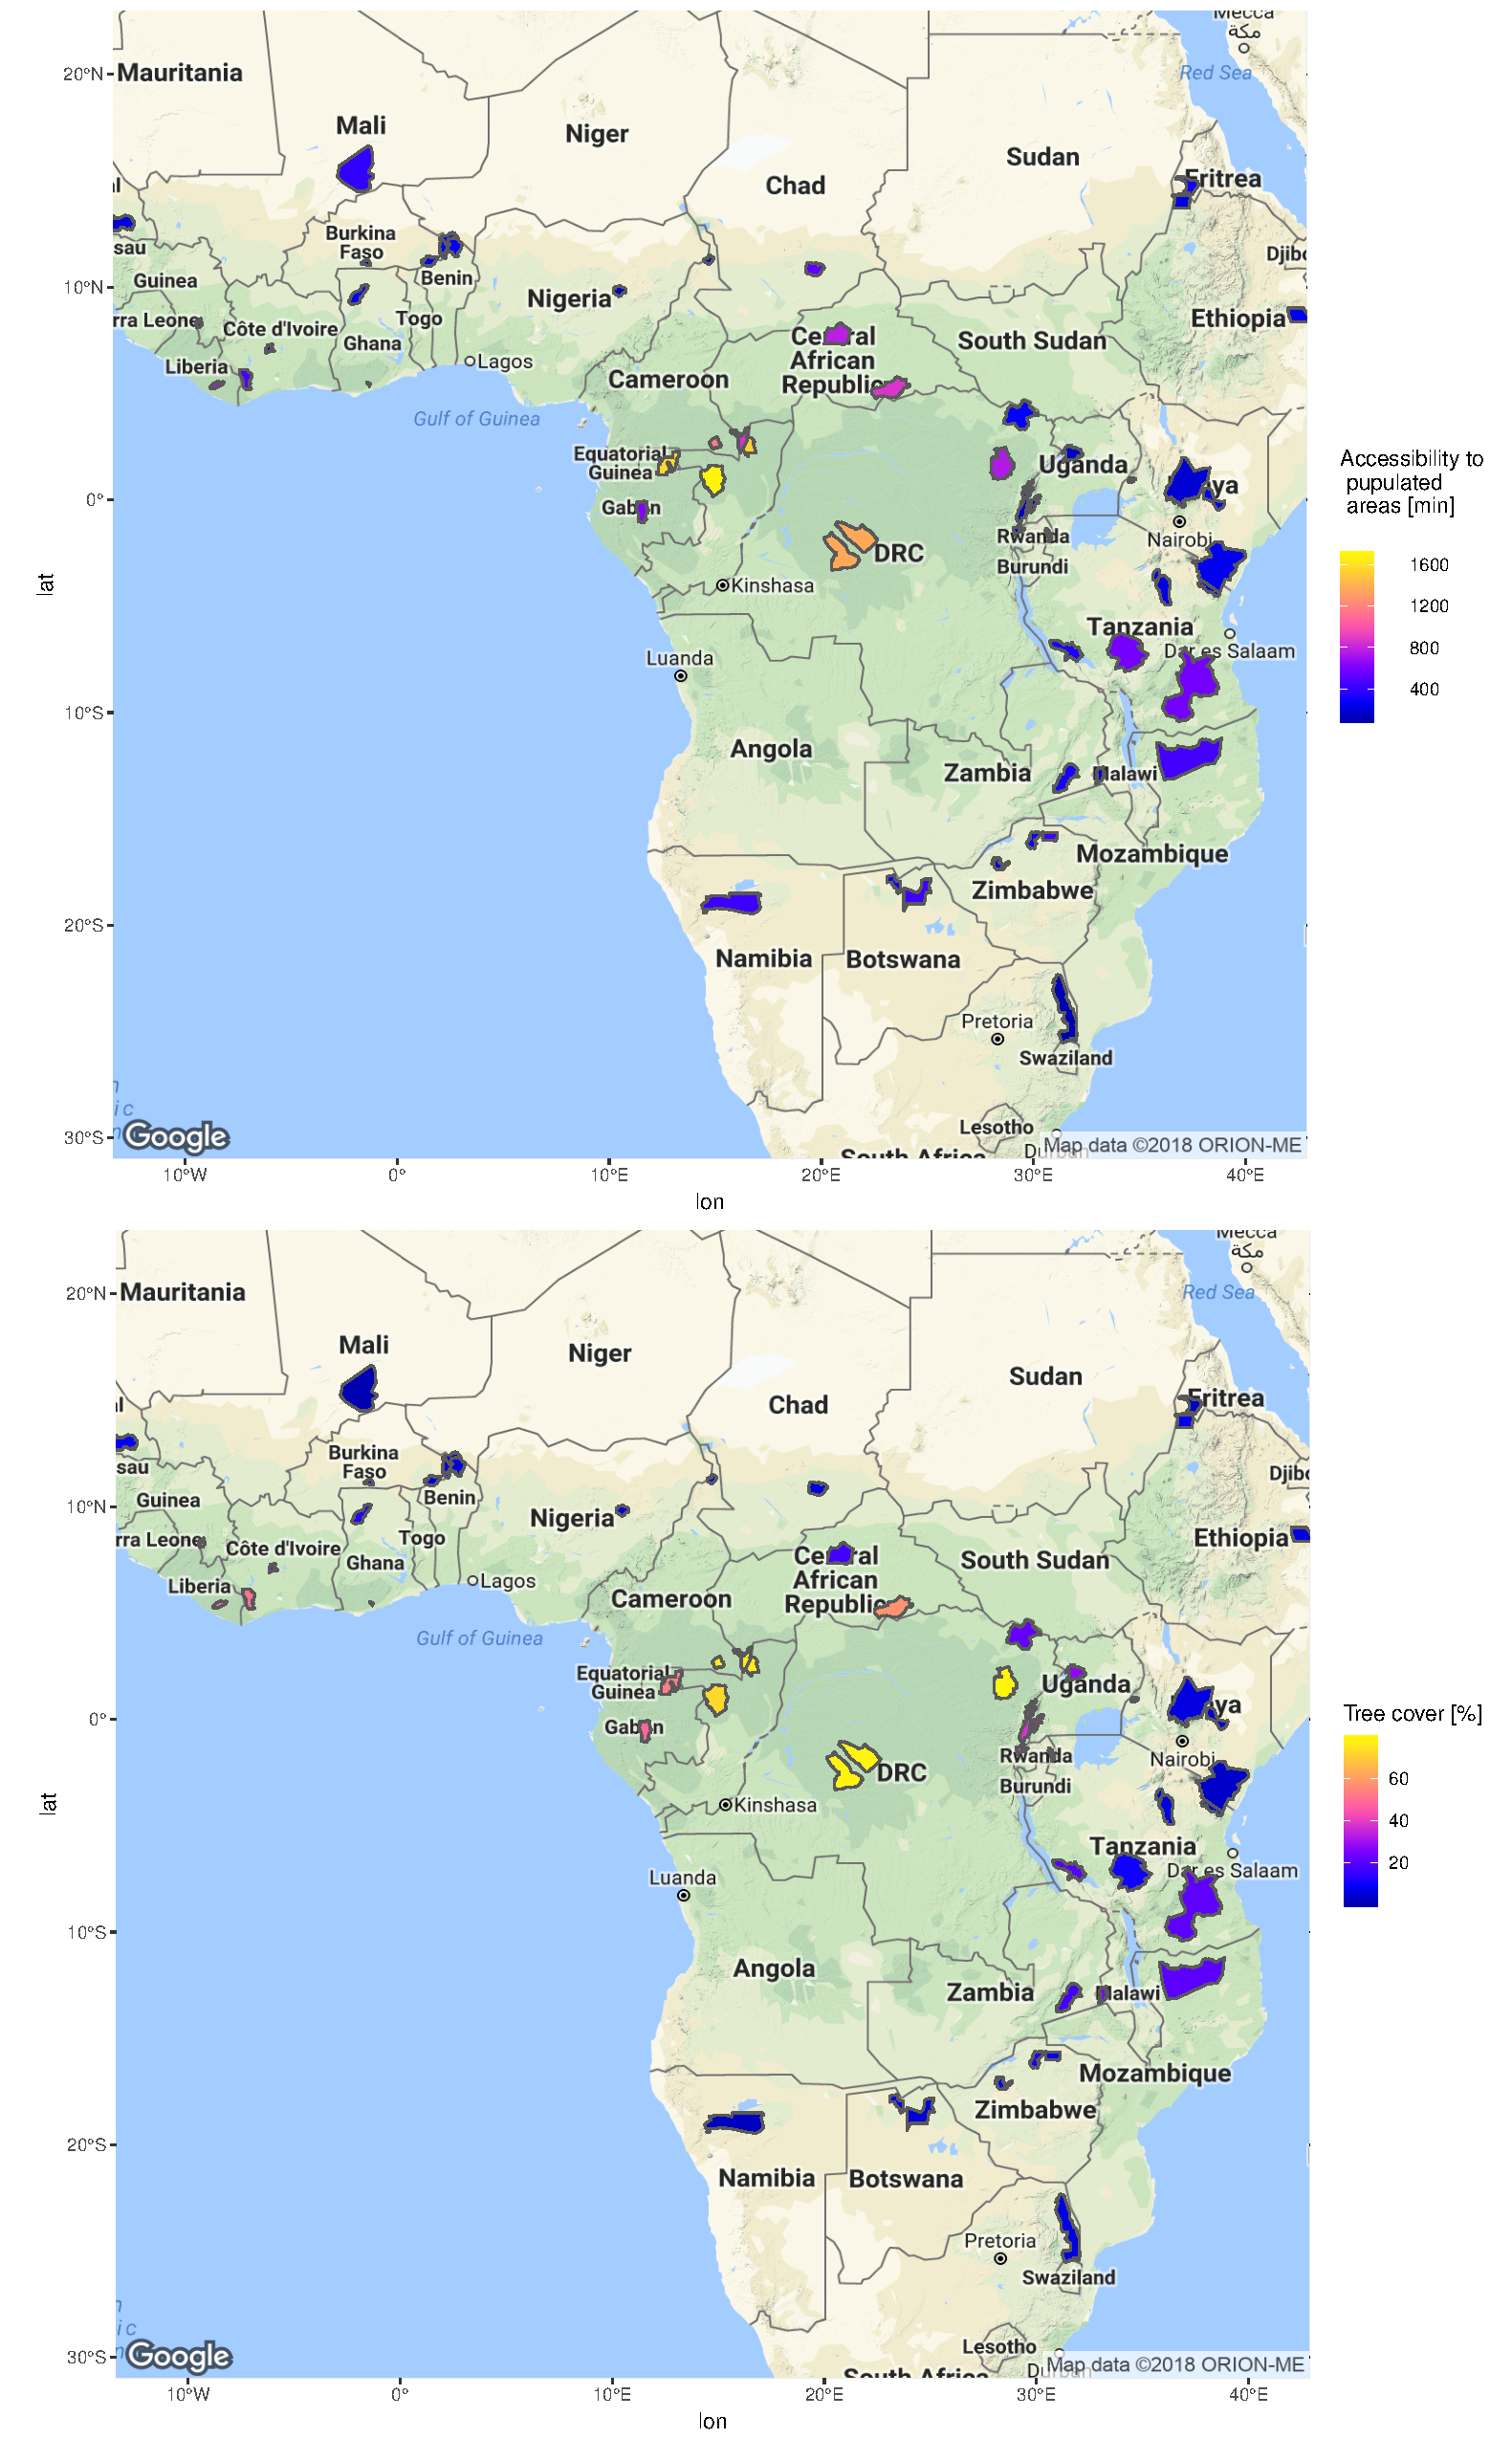
\includegraphics[width=14cm]{images/sample_session_1-cropped.pdf}
			\caption{on top the accessibility to the nearest populated areas in minutes and tree cover in percent at the bottom}
			\label{sample_session_1}
		\end{center}
	\end{figure}
	% \vskip 2em%
\end{center}


Figure \ref{sample_session_1} shows the mean tree cover in percent from 2000 to 2005 for each elephant territory in the upper figure and the mean accessibility of the territories in the figure at the bottom. Eye-catching but not surprising is the negative relationship between accessibility and tree cover resulting in a regional pattern with the highest tree cover and lowest accessibility found in central Africa, while toward the north, south and west, the accessibility increases and the tree cover decreases.

While this sample session shows the capabilities of the earthEngineGrabR package to aggregate over large areas, the next example is dedicated to the opposite situation. 

\section{Small-scale analysis}

\begin{wrapfigure}{r}{0.5\textwidth}
	\begin{center}
		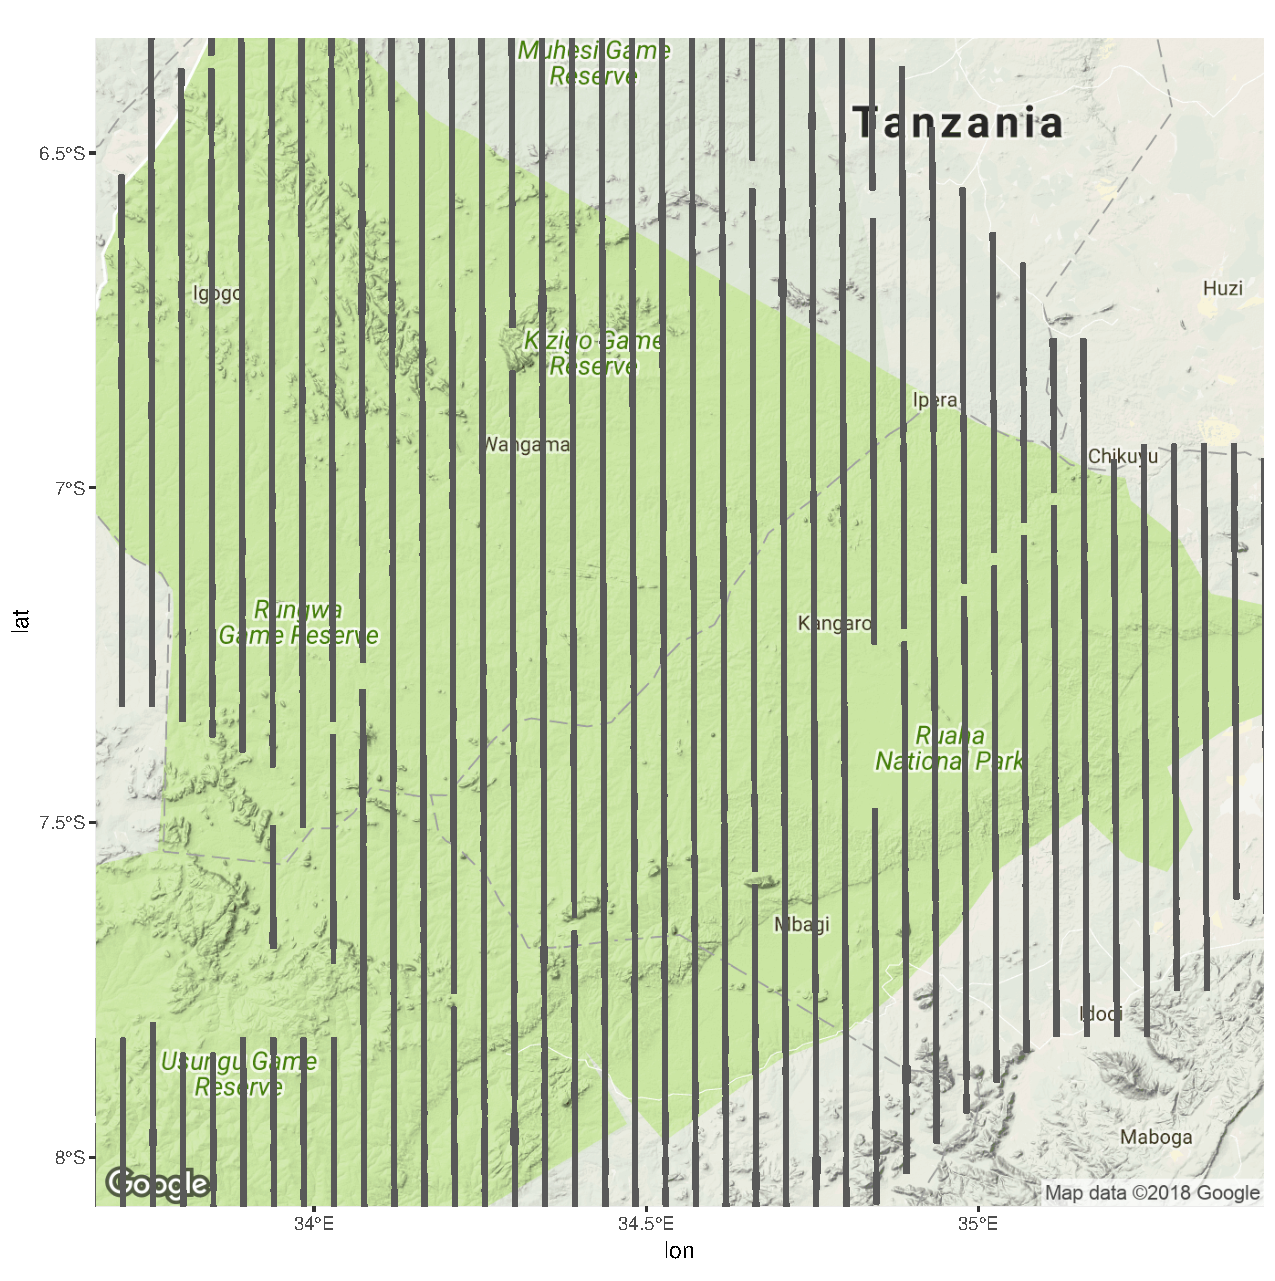
\includegraphics[width=7cm]{images/stripes-cropped.pdf}
		\caption{Spatial coverage of the aerial survey for Tanzania}
		\label{stripes}
	\end{center}
\end{wrapfigure}
% \vskip 2em%


Because of your access to the Great Elephant Census data you have not only the aggregated data for each territory but also the pre-aggregated survey data consisting of the number of elephants counted within a region specified by position, hight and the flight path of the aircraft. 


The combined areas form the spatial coverage of the survey and are available as shapefiles.
Figure \ref{stripes} shows the coverage for Tanzania. You are interested in the availability of surface water in each of these regions. Therefore you want to use the jrc-distance-to-surface-water data product available in the earthEngineGrabR package. 
As the target, you use the shapefile of the survey coverage and only specify the \texttt{jrc\_distanceToWater} product in the products argument. As spatial and temporal reducer you choose median. 

\begin{lstlisting}

africa_elephant_data_stripes <- ee_grab(
target = system.file("data/aerial-stripes.shp", package="earthEngineGrabR"), 
products = list(
eeProduct_jrc_distanceToWater(yearIntervall = c(2000,2000), spatialReducer = "median")
),
resolution = 50
)
\end{lstlisting}



Due to the smaller area of the features of the target (mean area of 0.7 km$^2$), you choose a resolution of 50 m and execute the function. The computation time takes about 3 m, and the result is shown in figure \ref{session_2}. Since the area of the coverage is too small for a meaningful visualisation, figure \ref{session_2} shows an actively zoomed view of the actual figure \ref{stripes}. 

\begin{center}
	\begin{figure}[h]
		\begin{center}
			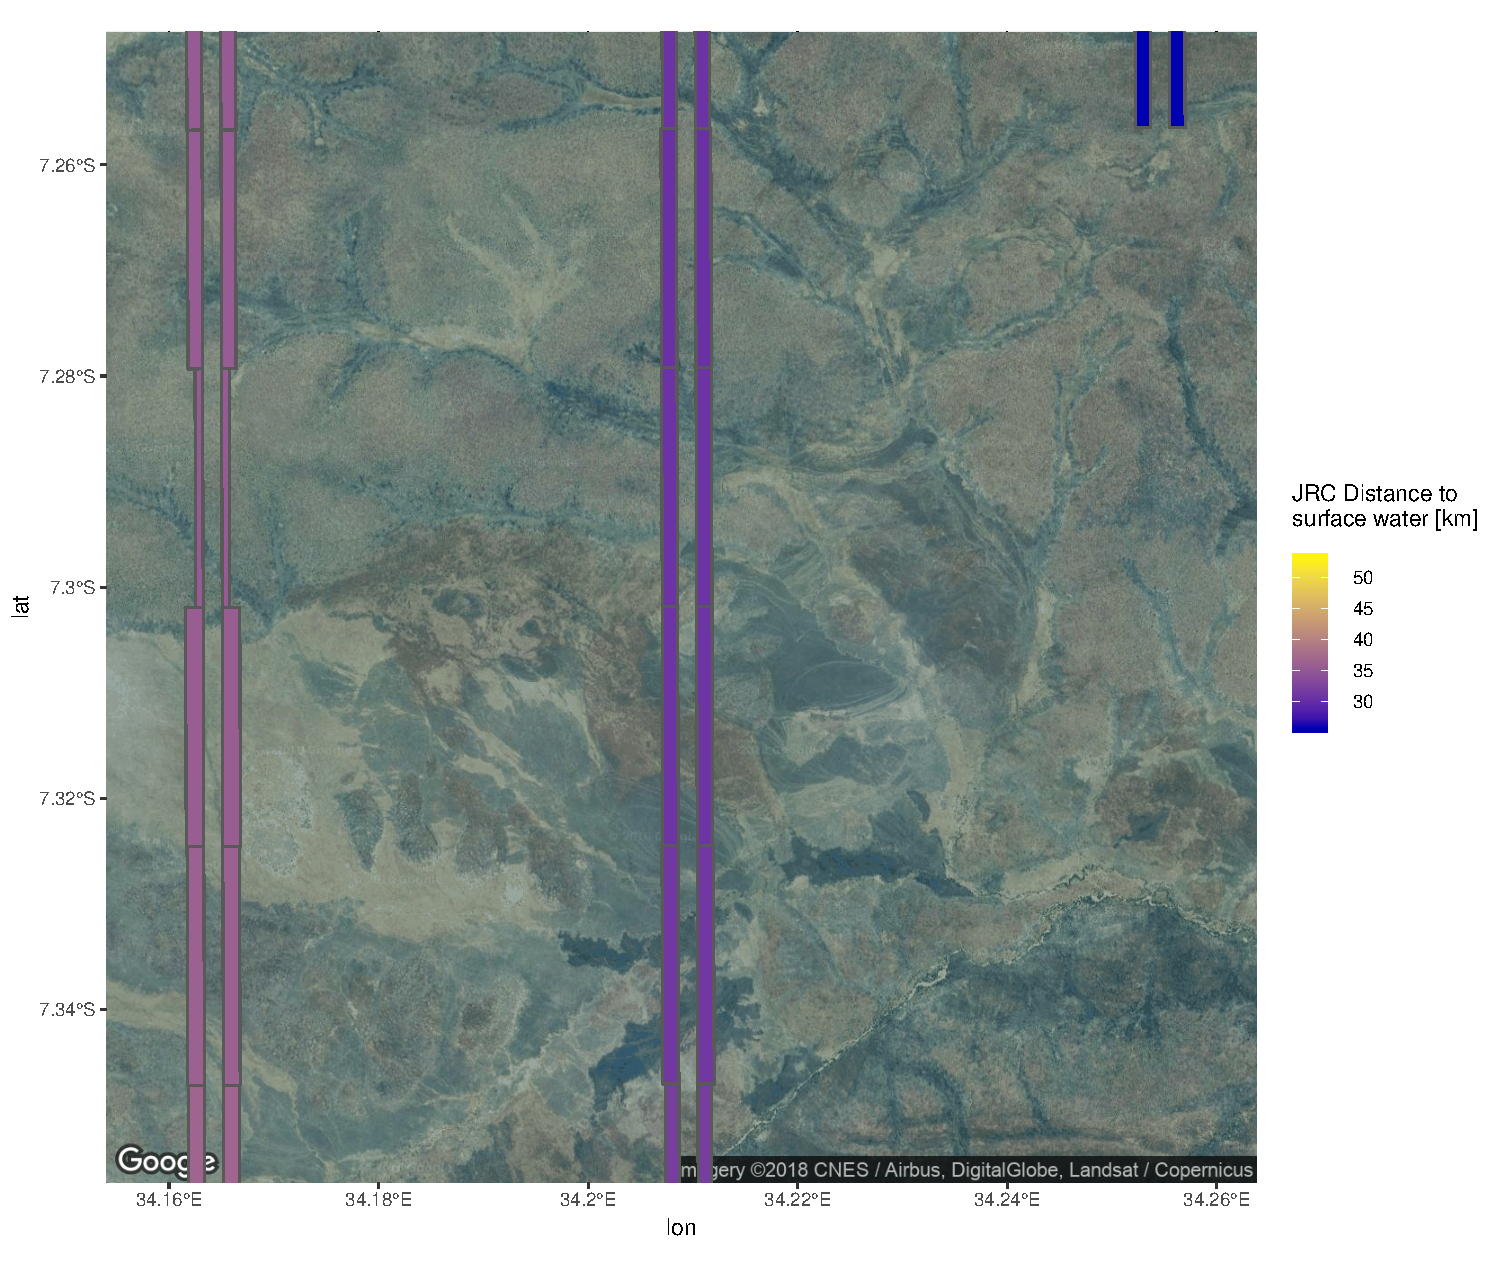
\includegraphics[width=15cm]{images/smalle-scale-analysis-cropped.pdf}
			\caption{Distance to surface water in km for the coverage of the areal survey}
			\label{session_2}
		\end{center}
	\end{figure}
	% \vskip 2em%
\end{center}

The distance to surface water is specified in km (though, the actual resolution is 50 m) and refers to the distance to the next Landsat pixel (30 m x 30 m) classified as water (\cite{pekel2016high}). The distance ranges from approximately 25 km to 35 km. In figure \ref{session_2} the aerial stripes on the left indicate a higher distance than the stripes on the right side of the map. Thus, the next close surface water must be located approximately 25 km in an eastward direction. 

This session shows the flexibility of the earthEngineGrabR referred to the scale of analysis and the shape of the AOI.

In the last example, a more extended use case of the \texttt{ee\_grab()} function is presented.

\section{Time-series analysis}

You are also interested in changes over time, for example, the change of precipitation in the elephant territories. Out of the documentation you know, that the precipitation product of the earthEngineGrabR is available from 2000 to 2015 on a yearly basis, thus you decide to calculate the precipitation for each year from 2000 to 2015 and analyse the change by using a linear model. The chirps-precipitation product is produced from satellite data on a daily basis, what offers the possibility to calculate the yearly precipitation sum. Because the yearly precipitation sum is a common practice in hydrology and compared to the mean not this prone to extreme values you decide to calculate the annual sum in each of the elephant territories for each year. To achieve that, you create one product for each year and pass the list of products to the \texttt{ee\_grab()} function.
The list of products can be generated using a vector of years from 2000 to 2015 and iterate the precipitation data product function over the years vector.

\begin{lstlisting}

years <- 2000:2015
products_ts <- list()

for (i in seq_along(years)) {
products_ts[[i]] <- eeProduct_chirps_precipitation(yearIntervall = c(years[i], years[i]), temporalReducer = "sum")
}

precipitation_time_series <- ee_grab(
target = system.file("data/territories.shp", package="earthEngineGrabR"),
products = products_ts,
resolution = 1000
)
\end{lstlisting}


As temporal reducer, you choose sum, and for the year interval, you take the i-th value of the created years vector. This generates a list of 15 specified data products for each year from 2000 to 2015. This list is passed to the products argument in the \texttt{ee\_grab()} function.
Due to the large-scale of your analysis, you again select a resolution of 1000 m. Since you want the spatial mean of the yearly precipitation sum in the territories, which already is the default spatial reducer, all necessary parameters in the \texttt{ee\_grab()} function are specified. While the processing of a single request for one year would take about 3 m, the processing time of all 15 data products require only approximately 15 m. Because the requests are sent and processed in parallel, the relationship of processing time and the number of requests is nonlinear. This point will be explained further in the discussion.

The output is an object of class sf that contains all properties of the original territories shapefile with 15 added columns for the precipitation sum of each year.
Next, you use a linear model of $year  \sim precipitation$ for each territory and retrieve the estimates for the effect of year. 

The estimates show the linear effect of year on the yearly precipitation sum in mm for each of the elephant territories. 
By joining the estimates with the spatial data of the territories, the estimates can be visualised spatially. 

\begin{center}
	\begin{figure}[h]
		\begin{center}
			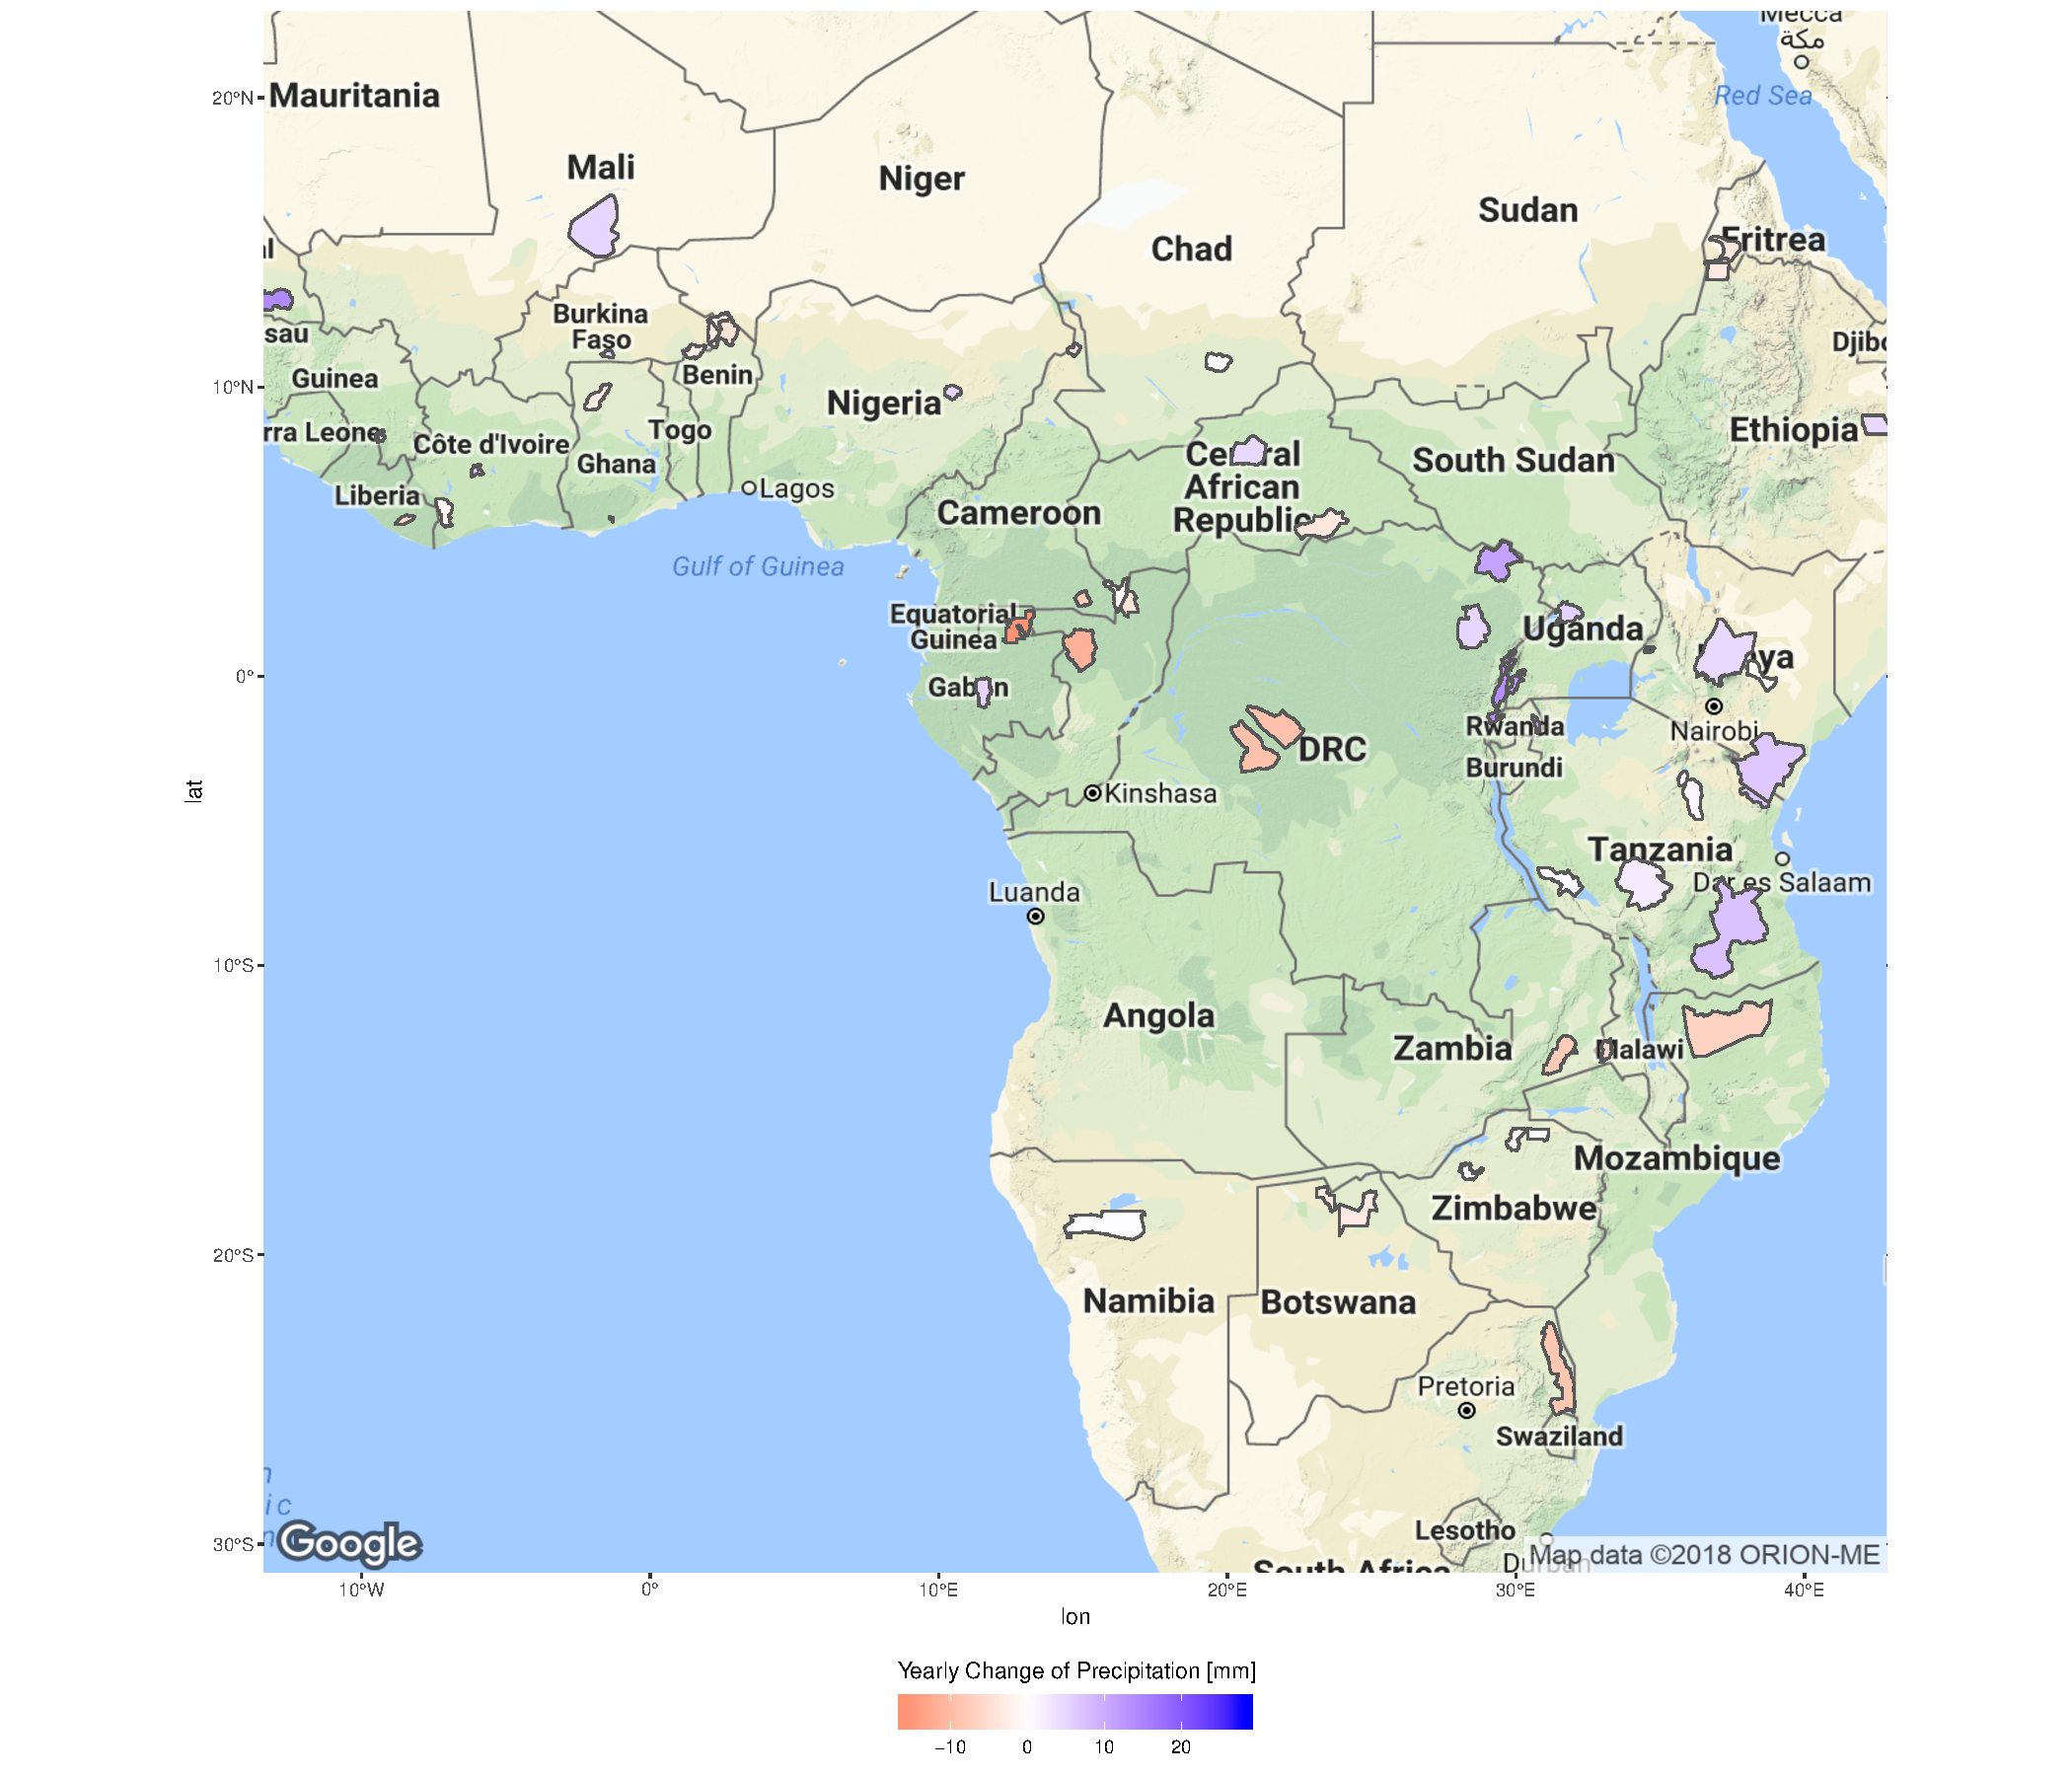
\includegraphics[width=16cm]{images/change_precipitation.pdf}
			\label{change}
		\end{center}
	\end{figure}
	% \vskip 2em%
\end{center}


Figure \ref{change} shows the estimate of the yearly change of the annual precipitation sum in mm for each territory. That estimates reflect a yearly change from - 10 mm to + 20 mm. While the yearly precipitation sum is increasing for the territories in East Africa, it is decreasing for most territories in central Africa, especially for those with hight tree cover (see figure \ref*{sample_session_1}).


\section{Summary}

The focus of this section is not on the interpretation of the results but to present the use of the earthEngineGrabR package.
With the use of the package, it was possible to quickly and easily acquire remote sensing data in three different use-cases. First, with the instructions on the packages Git Hup site, the requirements and the earthEngineGrabR were installed. Next, the \texttt{ee\_grab\_init()} installed the necessary Python dependencies and guided the user through the different authentications. The section illustrated how to use R, autocomplete feature and the package's data product functions to browse through the available data products and quickly open further documentation. Next, the \texttt{ee\_grab()} function was used to acquire remote sensing data according to 3 different questions and use-cases. The section showed the package's flexibility referring to the possible AOI, by obtaining data for both large-scale analyses with a mean area of the territories of 9862 km$^2$ and small-scale study with a mean area of 0.7 km$^2$.
The last sample session gave suggestions on how to extend the possibilities of the package by integrating the \texttt{ee\_grab()} over a series of years and doing this, acquire a time series of a specific data products.








\chapter{Discussion}


The previous sample sessions in the results section showed the ability of the earthEngineGrabR to acquire remote sensing data for various research questions.
Compared to the standard approach described in the introduction the earthEngineGrabR is superior in various ways:
The use of the earthEngineGrabR to acquire remote sensing data for a specific time, region and aggregation provide significant savings of time, processing resources and labour. To acquire, the data for the illustrated use-cases was a matter of minutes, even the aggregation of daily precipitation satellite imagery for 15 years required less than 15 m. The necessary processing resources for the computation was outsourced entirely, while there was only a minimum of load on the local processing resources. Further, no manual preprocessing or integration of different data sources was necessary, and no external GIS software had to be used. The entire process could be controlled from within R, and only a minimum of GIS knowledge and no experience with Python or the EE Python API was required. With the earthEngineGrabR, the user not only could harvest data products from the earth engine data catalogue but with the aggregation process controlled by the user, could generate new data dependent on the research questions. 

Therefore, for the described use cases, I can say that the earthEngineGrabR strongly simplified and at the same time extended the possibility of the user to acquire remote sensing data for there research questions. Further, the fast acquisition and preprocessing of the remote sensing data enables a more interactive excess to environmental variables.
Fast access to environmental variables enables fast descriptive analyses, and the test of various hypothesises before the modelling process.
Thereby, the package shows the potential of simplified access to the capabilities of EE for the scientific work.


\section{Limits and problems of the current version of the earthEngineGrabR}

Although in many cases, the use of the earthEngineGrabR package offers significant advantages to the scientific work, the current version is still limited in many ways. 

\subsubsection{Vector data processing restriction}

Mainly, due to the current upload limit of the Fusion Table API, it is not possible to process vector data with more than 5000 features. This small size certainly restricts the application of the package and would make it uncomely for most scientific projects. 

\subsubsection{Limited number of available data products and their possible properties}

Furthermore, the choice of available data products and their properties in the earthEngineGrabR is still low. The package, for example, offers no product for temperature, climate or any vegetation indexes and the available products lack a necessary temporal resolution. For instance, since the smallest temporal interval is one year, it is not possible to request the precipitation or distance to surface water for a particular season. However, for the most ecological problems, the seasonality is of great importance.

\subsubsection{No control of projection}

Another problem is, that during the upload process all vector data is transformed to geographic reference system WGS84. That is that all the processing in EE is performed without a projection unless you call the WGS84 a projection. Therefore all projections of the original vector data are lost. The output of the \texttt{ee\_grab()} function does not reflect the projection of the imported vector data. The conversion to WGS84 is unproblematic as long as there is no calculation of areas. Since the spatial reducer of the earthEngineGrabR only allows simple statistics like mean, median, mode, min and max, there is no calculation of areas, and the conversion is harmless to the results of the analysis. However, in most cases, it would require a manual reprojection of the results by the user to combine the data collected by the earthEngineGrabR with data that is already at hand. Additional control of the projection would be helpful.

\subsubsection{Multiple dependencies, operating system interoperability, confusing authentication process}

The most challenging problem though is to get the earthEngineGrabR to work on all operating systems properly. This point is challenging because of the many requirements and dependencies of the package and the approach to invoke system calls. There are dependencies to R packages python libraries and external libraries such as GDAL, and there has to be a working python distribution on the system (Table \ref{dependencies}). If any of the requirements are not met, the package crashes. 
Further, the invoked system calls depend on specified paths as environmental variables on the users operating system. For example the commands \texttt{python}, \texttt{pip} or \texttt{ogr2ogr} are invoked with the \texttt{system()} function, if the commands can't be found, the execution fails. The problems could be solved by specifying the full path to the underlying programmes, but these again depend on the operating system and the Python distribution that is installed. In summary, the approach to use invoked system call via R's \texttt{system()} functions makes the package vulnerable to internal errors due to interoperability of different operating systems and local environments.

An additional difficulty is the confusing and extensive authentication process. While the Google Drive and Fusion Table API are accessed directly with R, the EE API and the GDAL driver for Fusion Tables are accessed with Python. In R the authentication protocol is managed by the httr R package and requires no manual copying and pasting of authorisation tokens. For the authorisation to the API's accessed from Python the copy and pasting of tokens are still necessary. 
Furthermore, the httr R package in its current implementation of the earthEngineGrabR works with access tokens, which need to be refreshed after approximately an hour while the authentication protocols managed with different Python libraries work with refresh tokens, which never expire and therefore only need one initial authorisation. While using the earthEngineGrabR, this results in regular interruptions where the user is asked to again log in to his Google Account. Although with an already logged in account, this is just one click with a mouse per hour, this can be problematic for unsupervised use of the package for instance on a  server. Therefore, although already strongly simplified, the current management of the dependencies and authentication protocols is still error-prone and requires too much activity on the user's side.

\section{Further development of the earthEngineGrabR}

Most of the shortcomings addressed in the last section can be rectified with the further development of the earthEngineGrabR package. 

The further development can be divided into the improvement of the interface between R and EE and the implementation and of additional features.

\subsection{Implementation of additional features}

Below, some additional extensions to the earthEngineGrabR are described that will rectify most of the addressed shortcomings.

\subsubsection{Add more data products}

The most important extension is the implementation of additional data products. All data products available within the EE public data catalogue can be considered (Table \ref{app:appendix2}). To provide data products covering weather and climate variables, the implementation of additional products based on ASTER (Advanced Spaceborne Thermal Emission and Reflection Radiometer) and MODIS would be reasonable. Furthermore, a data product to provide vegetation indices calculated form Sentinel or Landsat satellite imagery would be interestingg.

\subsubsection{Extend the properties of the data products}
To provide a smaller temporal resolution, the package could implement an additional monthInterval parameter, which filters for specific months. This would result in the possibility to specify year and month of the interval of interest and allow to acquire the chirps-precipitation and jrc-distance-to-surface-water product in a monthly resolution.
Furthermore, it would be reasonable to choose the spatial resolution for each data product separately and add control over the projection of the analysis. 
The projection could be controlled by using the target projection and send it as a string that specifies the EPSG (European Petroleum Survey Group - list of codes for geographic reference systems) to the EE servers and reprojects the requested data. Another option would be to control the projection explicitly with an additional argument.

\subsubsection{Internal iterations as a workaround for the vector data processing restriction}

To increase the overall file size and the number of features of the target that can be processed it is necessary to build a workaround for internal limitations of the Earth Engine API and the Fusion Table API. One is the upload limit for Fusion Tables, of around 5000 features at a time and another an export limit of Earth Engine of about 100 000 features at a time to Google Drive. The workaround for both limitations is to subdivide the file, iterate over the request of each subdivision and finally join the subdivision results back together. In the Fusion Table API, it is possible to upload vector data as a new Fusion Table or add to an existing one. Therefore, in the beginning, the file could be subdivided into chunks, which don't exceed 5000 features. While the first chunk is used to upload a new Fusion Table, all additional chunks can be added in an iteration process. This existing Fusion Table is used as the target in EE. If the export exceeds 100 000 features, it is again subdivided into multiple requests, downloaded separately and joined during the import process in R. This approach would enable the processing of considerably larger vector data and furthermore make use of a performance gain achieved by parallelisation and iteration. 

\subsubsection{Simplify the authentication process}

To simplify the authentication process, it would be relevant to replace the manually copy and pasting of the authorisation tokens with an automatic transfer. Next, all authorisation processes should work with a refresh token which only requires one initial authorisation. The produced credentials refresh automatically without the intervention of the user. To further shield the user from the authorisation process it would be reasonable to incorporate the \texttt{ee\_grab\_init()} inside the \texttt{ee\_grab()} function and run the initialisation if the credentials cannot be found. This way, if the user calls the \texttt{ee\_grab()} function the first time, \texttt{ee\_grab\_init()} gets called and triggers the authorisation process. 

\subsubsection{Add the possibility for the user to add and define new data products}

Finally, it would be necessary to consider a possibility to add new data products by the user. To achieve this either the earthEngineGrabR has to provide a function that works with all datasets on the EE Data Catalog or provide detailed documentation on how to create data products while the user acts like a coworker that incorporate changes to the earthEngineGrabR using the version control system of GitHub. This two examples indeed are extremes of two different designs of the earthEngineGrabR and a solution should make use of both directions. In the broader sense, it is the question of how to provide extensibility to users. It seems necessary that the package maintainer implements demanded features. However, to supply tools, that the users can build the required data products himself is probably superior to one individual being responsible for the implementation of every request.
Independently of the different approaches of how to provide extensibility, several implementations would undoubtedly simplify the integration of additional features and the collaboration with other users of the earthEngineGrabR package. The first is, to provide comprehensive documentation with additional sample sessions, vignettes or tutorials. Next, to implement tests in the development workflow and use them for Continuous Integration (CI). Discarding, of the improved stability of the package, testing and CI would improve the collaboration with co-workers and simplify the publication of the earthEngineGrabR. 

\subsection{Improve the integration of R and Python}

To improve the framework for the base functionality of the earthEngineGrabR package the interface of R and Python could be further developed. Instead of an interface depending on the console which invoiced system calls in the way described in the methods section the new published reticulate package of r-studio could be used (\cite{reticulate}). The use of reticulate would offer some significant benefits. The reticulate package provides the translation of R and Python data types. The direct translation of data from R to Python would overdue the use of a flat file connection to pass parameters or processing info. Further, reticulate contains a multitude of helper functions that ease the use of R in combination with Python (\texttt{py\_available()}, for instance, checks for a Python version on the system). While the execution of Pythons scripts with a console, require the Python code organised as scripts, with reticulate it's possible to run Python code directly in R and arrange the code in smaller, more flexible chunks, what is essential when it comes to tools that provide the option to expand the earthEngineGrabR with additional data products and functionalities. The use of the reticulate package also would simplify the installation of python dependencies, because they can be performed in R (\texttt{py\_install()} installs python libraries). Finlay, replace the invoiced system calls would solve the problem due to missing environmental variables. Because, most system call commands like \texttt{python} and \texttt{pip} could be replaced with functions of the reticulate package, the internal paths of these commands is irrelevant for the execution. The retuculate package would manage the execution and provide interoperability for all operating systems.

In summary, the reticulate package provide a more precise, less error-prone and more flexible interface of R and Python then the currently implemented use of system calls.

\section{Internal strengths, weaknesses and limitations of EE and their incorporation in the earthEngineGrabR}

Besides the discussed limitation, there are also limitations of EE, which in contrast to the limitations of the earthEngineGrabR, can't be avoided by further development of the package. 
These inherent limitations have a strong influence on the operations that can be performed efficiently with the package.
Accessory to the suggested improvement of the interface between R and Python and the
implementation of additional features, the limitations and strengths of EE pretend a direction to the further development of the package.

A reason for EE's performance is its ability to distribute and manage complex computations across many machines efficiently. There is an almost linear relationship of throughput (pixels/sec) with the number of machines (\cite{gorelick2017google}).
Although EE can execute and manage extensive computations, the underlying infrastructure consists of clusters of low-end servers, and there is a hard limit on the amount of data that can be brought to any individual server. The current Remote procedure call (RPC) and caching system limit the size of an object to 100 MB. An option to configure machines in EE is not available.

Users can only express computations by using the parallel processing primitives provided in the EE client library, and some non-parallelizable operations just cannot be performed efficiently in this environment.

\subsubsection{Strengths of EE}

The architecture of EE performers well on per-pixel and finite neighbourhood operations such as band-math, morphological operations, spectral unmixing, template matching and texture analysis and can easily combine such operations in long chains (hundreds to thousands). 

Furthermore, it is also highly optimised for statistical operations
that can be applied to a collection of images, such as computing statistics on a time-series stack of images. This way, the EE can easily handle very deep stacks (i.e., millions of images; trillions of pixels). 

\subsubsection{Weaknesses and limitations of EE}

It performs poorly for non-local operations in which a local value can be affected by arbitrarily distant inputs, such as watershed analysis or clustering algorithms. Further due to the caching limit of 100 MB, operations that require a significant amount of data allocatable at the same time, such as training many machine learning models or operations that involve long-running iterative processes, such as finite element analysis or agent-based models cannot be performed efficiently. 

Another significant limitation is the export limit of the EE to Google Drive.
The EE provides data export to Google Drive and Google Cloud Platform (GCP). While the export to GCP is fast and works with extensive datasets, the export to Google Drive is limited to 2 GB and proportionally slow. Due to the reason, that outside the USA the always free tier of the GCP is not available, the export to Google Drive is the only free option. Discarding the official limit of 2 GB, it has shown that keeping the size of the export small,  speeds up the process dramatically while export files larger 1 GB can result in hours of computation time. 

\subsection{The optimal application of EE in the earthEngineGrabR}

\subsubsection{Support the internal distribution mechanism of EE by processing the data products in parallel}

During the development of the earthEngineGrabR, the experience was repeatedly made, that requests of smaller magnitude are processed fast and immediately while requests exceeding a certain magnitude in data throughput, result in unforeseeable long data processing. Unfortunately, due to the reason, that the EE system hides nearly every aspect of the computation from the user, the magnitude generating this bottleneck is not obvious. Hence, avoiding the bottleneck saves hours of computation time and also enables processes that otherwise result in errors referring to computation timeout or user memory limit exceeding. For example, processing all available data products and joining them in one request, given a target shapefile of 10.000 features, takes more than 1 hour of computation, while iterating over the data products with one request each, is a matter of a few minutes. This insight is reflected in the internal design of the earthEnigneGrabR. In the \texttt{ee\_grab()} function, each data product is processed individually. Furthermore, this approach allows processing the data products in parallel. This way, data bottlenecks, resulting in long exporting and computation time and eventually timeout errors are avoided. The performance of the earthEngineGrabR depends on EE's ability to distribute computation by an internal parallelisation mechanism efficiently. Operations that can't be efficiently scaled result in unforeseeable long processes and error and slow down the computation. By requesting the data products individually and in parallel, instead of joining the inter-products in EE, the package supports the internal distribution and parallelisation mechanism of EE.

\subsubsection{Instead of acquiring Big Data, process Big Data and acquire the results}

The export limit of 2 GB from EE to Google Drive actively restricts the possible download size. To download large data sets under such conditions is time-consuming error-prone. Because the internal processes of EE are shielded from the user, there is no possibility to inform the user about the internal processing state of the computation. The user would have to wait unseeingly long without any response and in case of an internal error for nothing.
Therefore, if the task is to download large data sets, the search and order tools are the better choice.
Splitting the exported file into smaller chunks, indeed speed up the export and computation time but only partly solve the underlining problem.
While the data that can be processed inside EE can become remarkably large, the data that can be exported is proportionally small.
However, what makes EE unique are the available resources to process the data before exporting. 
To avoid the described export limit, instead of exporting the raw raster data, the processing resources are used to aggregate the data inside EE.  The aggregation inside EE dramatically reduces the file size and speeds up the export. 
With the earthEngineGrabR, it is not possible to acquire big geospatial data but to process big geospatial data and acquire the results.
Considering this, using vector data as the output of the \texttt{ee\_grab()} function is more suitable because it provides a more flexible data format, which can adapt the shape of any AOI. Furthermore, compared to raster, it is smaller in size and therefore can be downloaded faster avoiding the export limit of EE. 

The limitation and strengths of the earthEngineGrabR arise from the weakness and strengths of EE. Therefore, the generated data products should correspond to EE capabilities. For images, this results in the use of per-pixel and finite neighbourhood operations such as band-math, morphological operations, spectral unmixing, template matching and texture analysis.

To use the full potential of EE, the earthEngineGrabR has to provide comfortable and user-friendly access to the capabilities of EE while using EE's internal strengths to offer a variety of data products.

EE's internal strengths could be used to generate a number of processing intensive data products. For example to calculate different vegetation indices's out of satellite data. This product, would enable to choose a time interval in months, maximum cloud cover to filter the image collection, whether to use Landsat or Sentinel imagery and the index that is to be calculated. The product could generate NDVI, Normalised Difference Water Index (NDWI), Enhanced Vegetation Index (EVI) or Normalized Difference Built-up Index (NDBI) out of high-resolution satellite data.








%\chapter*{Acknowledgements}

\label{ch:Acknowledgements}
\addcontentsline{toc}{chapter}{Acknowledgements}


Firstly, I would like to express my gratitude to my advisor Severin Hauenstein for the continuous support of this thesis, for his patience and motivation. His commitment helped and inspired me throughout the time of the thesis.

My thanks also go to my co-supervisor Mirko Mälicke who gave me vital technical support at the beginning.

Besides my advisors, I would like to thank Prof. Dr Carsten Dormann, for his encouragement during the thesis and especially for his time in many little and precious talks before. 
I further want to thank Dr.-Ing. Holger Weinacker who immediately agreed to be the second reader.

I want to thank my dear friends and companions in misfortune and happiness Simon and Samuel for there sympathy, knowledge and friendship.
Finally, I very much thank Julia Angstenberger for her strong and brave proofreading.

Last but not least, I want to thank my wonderful girlfriend Katharina for her understanding and caring support and apologise for all hours of tiredness, despair and inattention.









\printbibliography


% Insert the first appendix
\chapter{This is Appendix 1...}
\label{app:appendix1}

Put appendix text here


% Insert the second appendix

% insert a second appendix
\chapter{Appendix}
\label{app:appendix2}


\begin{table}[h]
	\tiny
	\begin{tabularx}{\textwidth}{lXXXX}
		\toprule
		\textbf{Dataset} & \textbf{Nominal resolution} & \textbf{Temporal granularity}  & \textbf{Temporal coverage}  & \textbf{Spatial coveragee} \\
		\hline
		Landsat & & & & \\
			Landsat 8 OLI/TIRS	&30 m	&16 day&	2013–Now&	Global\\
			Landsat 7 ETM +	&30 m	&16 day	&2000–Now&	Global\\
			Landsat 5 TM	&30 m	&16 day	&1984–2012&	Global\\
			Landsat 4–8 surface reflectance	&30 m	&16 day	& 1984–Now &	Global\\
		Sentinel & & & & \\        
		Sentinel 1 A/B  &10 m	&6 day	&2014–Now	&Global \\
		Sentinel 2A MSI  &10/20 m	&10 day&	2015–Now&	Global\\
		
		MODIS & & & & \\  
		
		  MOD08 atmosphere&	$1^\circ$ &	Daily	&2000–Now&	Global\\
		  MOD09 surface reflectance&	500 m&	1 day/8 day&	2000–Now&	Global\\
		  MOD10 snow cover&	500 m&	1 day&	2000–Now&	Global \\
		  MOD11 temperature and emissivity&	1000 m&	1 day/8 day&	2000–Now&	Global\\
		  MCD12 Land cover&	500 m	&Annual	&2000–Now	&Global \\
		  MOD13 Vegetation indices&	500/250 m	&16 day	&2000–Now&	Global\\
		  MOD14 Thermal anomalies  fire&	1000 m&	8 day&	2000–Now&	Global\\
		  MCD15 Leaf area index/FPAR&	500 m&	4 day&	2000–Now&	Global\\
		  MOD17 Gross primary productivity	&500 m&	8 day&	2000–Now&	Global\\
		  MCD43 BRDF-adjusted reflectance	&1000/500 m&	8 day/16 day&	2000–Now&	Global\\
		  MOD44 veg. cover conversion&	250 m&	Annual&	2000–Now&	Global\\
		  MCD45 thermal anomalies and fire	&500 m&	30 day&	2000–Now&	Global\\
		
		 ASTER	& & & & \\	
		 L1 T radiance	&15/30/90 m	&1 day&	2000–Now&	Global \\
		 Global emissivity	&100 m	&Once	&2000–2010&	Global \\
		  
		 Other imagery	& & & & \\		
		 PROBA-V top of canopy reflectance&	100/300 m&	2 day&	2013–Now&	Global\\
		 EO-1 hyperion hyperspectral radiance&	30 m&	Targeted&	2001–Now&	Global\\
		 DMSP-OLS nighttime lights&	1 km&	Annual&	1992–2013&	Global\\
		 USDA NAIP aerial imagery&	1 m	&Sub-annual	&2003–2015& 	CONUS\\
		 
		 Topography			& & & & \\		
		 Shuttle Radar Topography Mission&	30 m&	Single&	2000&	$60^\circ$ N–$54^\circ$ S\\
		 USGS National Elevation Dataset&	10 m&	Single&	Multiple&	United States\\
		 USGS GMTED2010&	$7.5''$&	Single	&Multiple&	$83^\circ$ N–$57^\circ$S\\
		 GTOPO30&	$30''$	&Single	&Multiple	&Global\\
		 ETOPO1	& $1'$ &	Single&	Multiple &	Global \\
		 
		 Landcover		& & & & \\			
		 GlobCover	&300 m	&Non-periodic	&2009&	90°N–65°S\\
		 USGS National Landcover Database&	30 m	&Non-periodic	&1992–2011&	CONUS\\
		 UMD global forest change&	30 m&	Annual	&2000–2014&	$80^\circ$ N–$57^\circ$ S\\
		 JRC global surface water&	30 m&	Monthly	&1984–2015	&$78^\circ$ N–$60^\circ$ S\\
		 GLCF tree cover&	30 m	&5 year	&2000–2010	&Global\\
		 USDA NASS cropland data layer&	30 m&	Annual&	1997–2015&	CONUS\\
		  
		 Weather, precipitation, atmosphere	& & & & \\				
		 Global precipitation measurement& 	$6'$& 	3 h	& 2014–Now& 	Global\\
		 TRMM 3B42 precipitation& 	$15'$& 	3 h	& 1998–2015	& $50^\circ$ N–$50^\circ$ S\\
		 CHIRPS precipitation& 	$3'$& 	5 day& 	1981–Now& 	$50^\circ$ N–$50^\circ$ S\\
		 NLDAS-2& 	$7.5'$& 	1 h	& 1979–Now	& North America\\
		 GLDAS-2& 	$15'$& 	3 h	& 1948–2010	& Global\\
		 NCEP reanalysis& 	$2.5^\circ$ & 	6 h	& 1948–Now& 	Global\\
		 ORNL DAYMET weather& 	1 km& 	Annual& 1980–Now& 	North America\\
		  
		 GRIDMET&	4 km&	1 day&	1979–Now&	CONUS\\
		 NCEP global forecast system&	$15'$&	6 h&	2015–Now&	Global\\
		 NCEP climate forecast system&	$12'$	&6 h&	1979–Now&	Global\\
		 WorldClim	&$3''$ &	12 images&	1960–1990&	Global\\
		 NEX downscaled climate projections&	1 km&	1 day&	1950–2099&	North America\\
		 Population		& & & & \\		
		 WorldPop	&100 m	&5 year	&Multiple	& 2010–2015\\
		 GPWv4	& $30''$ &	5 year&	2000–2020&	$85^\circ$ N–$60^\circ$ S\\
		\bottomrule
	\end{tabularx}
	\caption{Frequently used datasets in the earth engine data catalog (\cite{gorelick2017google})}
	\label{dependencies}
\end{table}



% If you used the makeidx package to create an index then use the 
% following command to print the index
\printindex

\chapter*{Selbstständigkeitserklärung} % (in German!)

\vspace{2cm}

\section*{Erklärung}

Ich versichere hiermit, dass ich die vorliegende Arbeit ohne fremde Hilfe selbstständig verfasst und nur die angegebenen Quellen und Hilfsmittel benutzt habe. Wörtlich oder dem Sinn nach aus anderen Werken entnommene Stellen habe ich unter Angabe der Quellen kenntlich gemacht.

\medskip
\noindent (I hereby declare that I have composed this document unassistedly and that I only used the sources and devices I declared. Passages taken verbatim or in meaning from other sources are identified as such and the sources are acknowledged and cited.)

\vspace{2cm}

\noindent \year

\end{document}